%%%%%%%%%%%%%%%%%%%%%%%%%%%%%%%%%%%%%%%%%%%%%%%%%%%%%%%%%%
%   Autoren:
%   Prof. Dr. Bernhard Drabant
%   Prof. Dr. Dennis Pfisterer
%   Prof. Dr. Julian Reichwald
%%%%%%%%%%%%%%%%%%%%%%%%%%%%%%%%%%%%%%%%%%%%%%%%%%%%%%%%%%

%%%%%%%%%%%%%%%%%%%%%%%%%%%%%%%%%%%%%%%%%%%%%%%%%%%%%%%%%%
%	ANLEITUNG: 
%   1. Ersetzen Sie firmenlogo.jpg im Verzeichnis img
%   2. Passen Sie alle Stellen im Dokument an, die mit 
%      @stud 
%      markiert sind 
%%%%%%%%%%%%%%%%%%%%%%%%%%%%%%%%%%%%%%%%%%%%%%%%%%%%%%%%%%

%%%%%%%%%%%%%%%%%%%%%%%%%%%%%%%%%%%%%%%%%%%%%%%%%%%%%%%%%%
%	ACHTUNG: 
%   Für das Erstellen des Literaturverzeichnisses wird das 
%   modernere Paket biblatex in Kombination mit biber 
%   verwendet - nicht mehr das ältere Paket BibTex!
%
%   Bitte stellen Sie Ihre TeX-Umgebung entsprechend ein (z.B. TeXStudio): 
%   Einstellungen --> Erzeugen --> Standard Bibliographieprogramm: biber
%%%%%%%%%%%%%%%%%%%%%%%%%%%%%%%%%%%%%%%%%%%%%%%%%%%%%%%%%%

\documentclass[fontsize=11pt,BCOR=5mm,DIV=13,parskip=half,listof=totoc,
               paper=a4,toc=bibliography,pointlessnumbers]{scrreprt}



               
\usepackage[utf8]{inputenc}

%% LANGUAGE SETTINGS
%
% @stud: Sprache ggf. anpassen
%
\usepackage[ngerman]{babel} 	        % german language
\usepackage[german=quotes]{csquotes} 	% correct quoting using \enquote{}

%%%%%%%%%%%%%
%% ZITIERSTIL
%%%%%%%%%%%%%
%
% @stud: Zitierstil in package biblatex unten wählen
%
% NUMERIC Style - e. g. [12]
% style=numeric 
%
% IEEE Style - numeric kind of style 
% style=ieee 
%
% ALPHABETIC Style - e. g. [AB12]
% style=alphabetic 
%
% HARVARD Style 
% style=apa 
%
% CHICAGO Style 
%style=authoryear
%
% Position des Zitats:
%
% autocite=inline 
%
% (!!) FOOTNOTE POSITION NOT RECOMMENDED IN MINT DOMAIN:
% autocite=footnote
%
\usepackage[backend=biber, autocite=inline, style=authoryear]{biblatex} 	
\usepackage{makeidx}                  % allows index generation
\usepackage{listings}	                %Format Listings properly
\usepackage{lipsum}                   % Blindtext
\usepackage{graphicx}                 % use various graphics formats
\usepackage[german]{varioref}         % nicer references \vref
\usepackage{caption}	                % better Captions
\usepackage{booktabs}                 % nicer Tabs
\usepackage[hidelinks=true]{hyperref} % keine roten Markierungen bei Links
\usepackage{fnpct}                    % Correct superscripts 
\usepackage{calc}                     % Used for extra space below footsepline, in particular
\usepackage{array}
\usepackage{acronym}
\usepackage{algorithm}
\usepackage{algpseudocode}
\usepackage{setspace}
\usepackage{tocloft}
\usepackage[T1]{fontenc}

% Definitionen und Commands
\newcommand{\indextype}{numeric}
\newcommand{\abs}{\par\vskip 0.2cm\goodbreak\noindent}
\newcommand{\nl}{\par\noindent}
\newcommand{\mcl}[1]{\mathcal{#1}}
\newcommand{\nowrite}[1]{}
\newcommand{\NN}{{\mathbb N}}
\newcommand{\imagedir}{img}
\newcommand{\TitelDerArbeit}[1]{\def\DerTitelDerArbeit{#1}\hypersetup{pdftitle={#1}}}
\newcommand{\AutorDerArbeit}[1]{\def\DerAutorDerArbeit{#1}\hypersetup{pdfauthor={#1}}}
\newcommand{\Firma}[1]{\def\DerNameDerFirma{#1}}
\newcommand{\Kurs}[1]{\def\DieKursbezeichnung{#1}}
\newcommand{\Abteilung}[1]{\def\DerNameDerAbteilung{#1}}
\newcommand{\Studiengangsleiter}[1]{\def\DerStudiengangsleiter{#1}}
\newcommand{\WissBetreuer}[1]{\def\DerWissBetreuer{#1}}
\newcommand{\FirmenBetreuer}[1]{\def\DerFirmenBetreuer{#1}}
\newcommand{\Bearbeitungszeitraum}[1]{\def\DerBearbeitungszeitraum{#1}}
\newcommand{\Abgabedatum}[1]{\def\DasAbgabedatum{#1}}
\newcommand{\Matrikelnummer}[1]{\def\DieMatrikelnummer{#1}}
\newcommand{\Studienrichtung}[1]{\def\DieStudienrichtung{#1}}
\newcommand{\ArtDerArbeit}[1]{\def\DieArtDerArbeit{#1}}
\newcommand{\Literaturverzeichnis}{Literaturverzeichnis}

% Page Layout
%\oddsidemargin=0mm
%\evensidemargin=0mm
%\textwidth=159mm
%\topmargin=-18mm
%\headsep=10mm
%\textheight=251mm
%\footheight=15mm

\makeindex

%%%%%%%%%%%%%%%%%%%%%%%%%%%%%%%%%%%
% LITERATURVERZEICHNIS
% @stud: Literaturverzeichnis in Datei bibliography.bib anpassen. 
%
% [Alternative zu Verwendung von \initializeBibliography: Citavi ... (dazu eigenes LaTex Coding verwenden)]
%
\addbibresource{bibliography.bib}
\DefineBibliographyStrings{ngerman}{andothers = {{et\,al\adddot}},}

% Elementare Konfigurationen und Definitionen werden geladen 
% @stud: gegebenenfalls anpassen
%
% !TEX root =  master.tex

%%%%%%%%%%%%%%%%%%%%%%%%%%%%%%%%%%%%%%%%%%%%%%%%%%%%%%%%%%%%%%%%%%
%	ANLEITUNG: 
% Passen Sie gegebenenfalls alle Stellen im Dokument an, die mit 
% @stud 
% markiert sind.
%%%%%%%%%%%%%%%%%%%%%%%%%%%%%%%%%%%%%%%%%%%%%%%%%%%%%%%%%%%%%%%%%%

%%
%% @stud
%%
%% LANGUAGE SETTINGS
\usepackage[ngerman]{babel} 	        % german language
\usepackage[german=quotes]{csquotes} 	% correct quoting using \enquote{}
%\usepackage[english]{babel}          % english language
%\usepackage{csquotes} 	              % correct quoting using \enquote{}

\usepackage{makeidx}                  % allows index generation
\usepackage{listings}	                %Format Listings properly
\usepackage{lipsum}                   % Blindtext
\usepackage{graphicx}                 % use various graphics formats
\usepackage[german]{varioref}         % nicer references \vref
\usepackage{caption}	                % better Captions
\usepackage{booktabs}                 % nicer Tabs
\usepackage[hidelinks=true]{hyperref} % keine roten Markierungen bei Links
\usepackage{fnpct}                    % Correct superscripts 
\usepackage{calc}                     % Used for extra space below footsepline, in particular
\usepackage{array}
\usepackage{acronym}
\usepackage{algorithm}
\usepackage{algpseudocode}
\usepackage{setspace}
\usepackage{tocloft}
\usepackage{rotating}

%% Schriftarten- und Zeichenpakete
\usepackage[T1]{fontenc}
\usepackage[utf8]{inputenc}


%%
%% @stud
%%
%%	FONT SELECTION: Schriftarten und Schriftfamilie
%%%%%%%%%%%%%
%% SCHRIFTART
%%%%%%%%%%%%%
% 0) without decomment: normal font families 
% ...
% 1) Latin Modern 
\usepackage{lmodern}        
% 2) Times 
%\usepackage{mathptmx}         
% 3) Helvetica
%\usepackage[scaled=.92]{helvet} 
%%%%%%%%%%%%%%%%%%
%%	SCHRIFTFAMILIE
%%%%%%%%%%%%%%%%%%
% ohne Serifen
\renewcommand*{\familydefault}{\sfdefault}
\addtokomafont{disposition}{\sffamily}
%
% mit Serifen
%\renewcommand*{\familydefault}{\rmdefault}
%\addtokomafont{disposition}{\rmfamily}
%
% Typewriter
%\renewcommand*{\familydefault}{\ttdefault}
%\addtokomafont{disposition}{\ttfamily}

%%
%% @stud
%%
%% Uncomment the following lines to support hard URL breaks in bibliography 
%\apptocmd{\UrlBreaks}{\do\f\do\m}{}{}
%\setcounter{biburllcpenalty}{9000}% Kleinbuchstaben
%\setcounter{biburlucpenalty}{9000}% Großbuchstaben

%%
%% @stud
%%
%% FOOTNOTES: Count footnotes over chapters
\counterwithout{footnote}{chapter}

%	ACRONYMS
\makeatletter
\@ifpackagelater{acronym}{2015/03/20}
{\renewcommand*{\aclabelfont}[1]{\textbf{{\acsfont{#1}}}}}{}
\makeatother

%	LISTINGS
% @stud: ggf. Namen/Text anpassen (englisch)
\renewcommand{\lstlistingname}{Quelltext} 
\renewcommand{\lstlistlistingname}{Quelltextverzeichnis}
\lstset{numbers=left,
	numberstyle=\tiny,
	captionpos=b,
	basicstyle=\ttfamily\small}

%	ALGORITHMS
% @stud: ggf. Namen/Text anpassen (englisch)
\renewcommand{\listalgorithmname}{Algorithmenverzeichnis}
\floatname{algorithm}{Algorithmus}

%	PAGE HEADER / FOOTER
%	Warning: There are some redefinitions throughout the master.tex-file!  DON'T CHANGE THESE REDEFINITIONS!
\RequirePackage[automark]{scrlayer-scrpage}
%alternatively with separation lines: \RequirePackage[automark,headsepline,footsepline]{scrlayer-scrpage}

\renewcommand{\chaptermarkformat}{}
\RedeclareSectionCommand[beforeskip=0pt]{chapter}
\clearpairofpagestyles

%\ifoot[\rule{0pt}{\ht\strutbox+\dp\strutbox}DHBW Mannheim]{\rule{0pt}{\ht\strutbox+\dp\strutbox}DHBW Mannheim}
\ofoot[\rule{0pt}{\ht\strutbox+\dp\strutbox}\pagemark]{\rule{0pt}{\ht\strutbox+\dp\strutbox}\pagemark}
\ohead{\headmark}

\providecommand{\TitelDerArbeit}[1]{\def\DerTitelDerArbeit{#1}\hypersetup{pdftitle={#1}}}
\providecommand{\AutorDerArbeit}[1]{\def\DerAutorDerArbeit{#1}\hypersetup{pdfauthor={#1}}}
\providecommand{\Firma}[1]{\def\DerNameDerFirma{#1}}
\providecommand{\Kurs}[1]{\def\DieKursbezeichnung{#1}}
\providecommand{\Abteilung}[1]{\def\DerNameDerAbteilung{#1}}
\providecommand{\Studiengangsleiter}[1]{\def\DerStudiengangsleiter{#1}}
\providecommand{\WissBetreuer}[1]{\def\DerWissBetreuer{#1}}
\providecommand{\FirmenBetreuer}[1]{\def\DerFirmenBetreuer{#1}}
\providecommand{\Bearbeitungszeitraum}[1]{\def\DerBearbeitungszeitraum{#1}}
\providecommand{\Abgabedatum}[1]{\def\DasAbgabedatum{#1}}
\providecommand{\Matrikelnummer}[1]{\def\DieMatrikelnummer{#1}}
\providecommand{\Studienrichtung}[1]{\def\DieStudienrichtung{#1}}
\providecommand{\ArtDerArbeit}[1]{\def\DieArtDerArbeit{#1}}
\providecommand{\Literaturverzeichnis}{Literaturverzeichnis}

\newcommand{\settingBibFootnoteCite}{
	\setlength{\bibparsep}{\parskip}		  % Add some space between biblatex entries in the bibliography
	\addbibresource{bibliography.bib}	    % Add file bibliography.bib as biblatex resource
	\DefineBibliographyStrings{ngerman}{andothers = {{et\,al\adddot}},}
}

\newcommand{\setTitlepage}{
	% !TEX root =  master.tex
% @stud: ggf. Namen/Text anpassen (englisch)
\begin{titlepage}
\begin{minipage}{\textwidth}
		\vspace{-2cm}
		\noindent 
\includegraphics[scale=0.25]{\imagedir/firmenlogo.jpg} \hfill 
\includegraphics{\imagedir/logo.jpg}
\end{minipage}
\vspace{1em}
%\sffamily
\begin{center}
	{\textsf{\large Duale Hochschule Baden-W\"urttemberg Mannheim}}\\[4em]
	{\textsf{\textbf{\large{\DieArtDerArbeit}arbeit}}}\\[6mm]
	{\textsf{\textbf{\Large{}\DerTitelDerArbeit}}} \\[1.5cm]
	{\textsf{\textbf{\large{}Studiengang Wirtschaftsinformatik}}\\[6mm]
	\textsf{\textbf{Studienrichtung \DieStudienrichtung}}}\vspace{10em}
	
	\begin{minipage}{\textwidth}
		\begin{tabbing}
		Wissenschaftliche(r) Betreuer(in): \hspace{0.85cm}\=\kill
		Verfasser(in): \> \DerAutorDerArbeit \\[1.5mm]
		Matrikelnummer: \> \DieMatrikelnummer \\[1.5mm]
		Firma: \> \DerNameDerFirma  \\[1.5mm]
		Abteilung: \> \DerNameDerAbteilung \\[1.5mm]
		Kurs: \> \DieKursbezeichnung \\[1.5mm]
		Studiengangsleiter: \> \DerStudiengangsleiter \\[1.5mm]
		Wissenschaftliche(r) Betreuer(in): \> \DerWissBetreuer \\[1.5mm]
		Firmenbetreuer(in): \> \DerFirmenBetreuer \\[1.5mm]
		Bearbeitungszeitraum: \> \DerBearbeitungszeitraum\\[1.5mm]
%		alternativ:\\[1.5mm]
%		Eingereicht: \> \DasAbgabedatum	
		\end{tabbing}
	\end{minipage}
\end{center}
\end{titlepage}
	\pagenumbering{roman} % Römische Seitennummerierung
	\normalfont	
}

\newcommand{\initializeText}{
	\clearpage
	\ihead{\chaptername~\thechapter} % Neue Header-Definition
	\pagenumbering{arabic}           % Arabische Seitenzahlen
}

\newcommand{\initializeBibliography}{
	\ihead{}
	\printbibliography[title=\Literaturverzeichnis] 
	\cleardoublepage
}

\newcommand{\initializeAppendix}{
	\appendix
  \ihead{}
  \cftaddtitleline{toc}{chapter}{Anhang}{}
}

% @stud
%
% PERSÖNLICHE ANGABEN (BITTE VOLLSTÄNDIG EINGEBEN zwischen den Klammern: {...})
%
\ArtDerArbeit{Projekt} 
\TitelDerArbeit{Entwicklung eines KI-basierten Chatbots: Anwendung und Implementierung bei Freudenberg \& Co. KG}
\AutorDerArbeit{Sean Tyler Straub}
\Abteilung{Corporate IT}
\Firma{Freudenberg \& Co. KG}
\Kurs{WWI22SEA}
\Studienrichtung{Software Engineering}
\Matrikelnummer{1009196}
\Studiengangsleiter{Prof. Dr. Henning Pagnia}
\WissBetreuer{Prof. Dr. Henning Pagnia}
\FirmenBetreuer{Simon Jarke}
\Bearbeitungszeitraum{06.05.2024 -- 25.08.2024}
\Abgabedatum{dd.mm.yyyy}

\begin{document}

\setTitlepage


%	Kurzfassung / Abstract
% @stud: abstract.tex bearbeiten
\chapter*{Kurzfassung (Abstract)}
\addcontentsline{toc}{chapter}{Kurzfassung (Abstract)}

Diese Projektarbeit widmet sich der Entwicklung und Implementierung eines auf \ac{KI} basierenden Chatbots bei \ac{FCO}.
Ziel des Projekts ist es, die Effizienz innerhalb der \ac{CIT} Abteilung durch den Einsatz moderner \ac{KI}-Technologien signifikant zu steigern.
Im Rahmen dieser Arbeit wird eine umfassende Analyse gruppenweiter Anwendungsfälle durchgeführt, um spezifische Anforderungen von \ac{FCO} zu identifizieren.

Zur optimalen Umsetzung des Projekts werden verschiedene Large Language Models und Embedding-Modelle auf der SAP \ac{BTP} evaluiert.
Dabei stehen insbesondere die Kriterien Antwortqualität, Antwortzeit und Kosten im Fokus, welche durch die Ergebnisse eine Umfrage unter internen Nutzern gewichtet wurden.
Auf Basis der Analyse erweisen sich das Large Language Model \textit{LLaMA3-70b} und das Embedding-Modell \textit{text-embedding-3-large} als die am besten geeigneten Optionen.

Anschließend erfolgt die Implementierung eines internen Chatbots mithilfe von SAP AI Core, der in der Lage ist, präzise und effiziente Antworten auf spezifische Anfragen zu liefern.
Der Chatbot soll den Arbeitsalltag der Kollegen erleichtern und langfristig einen wertvollen Beitrag zur Verbesserung der internen Prozesse bei \ac{FCO} leisten.
  
\cleardoublepage


%%%%%%%%%%%%%%%%%%%%%%%%%%%%%%%%%%%
% EHRENWÖRTLICHE ERKLÄRUNG
%
% @stud: ewerkl.tex bearbeiten
%
% !TEX root =  master.tex
\clearpage
\chapter*{Ehrenwörtliche Erklärung}

% Wird die folgende Zeile auskommentiert, erscheint die ehrenwörtliche
% Erklärung im Inhaltsverzeichnis.

% \addcontentsline{toc}{chapter}{Ehrenwörtliche Erklärung}
Ich versichere hiermit, dass ich die vorliegende Arbeit mit dem Titel \enquote{\textit{\DerTitelDerArbeit}} selbstständig verfasst und 
keine anderen als die angegebenen Quellen und Hilfsmittel benutzt habe. Ich versichere zudem, dass die eingereichte elektronische 
Fassung mit der gedruckten Fassung übereinstimmt.

\vspace{3cm}
Hockenheim, 06.11.2024 \hfill \DerAutorDerArbeit
 
\cleardoublepage  
%%%%%%%%%%%%%%%%%%%%%%%%%%%%%%%%%%%

%%%%%%%%%%%%%%%%%%%%%%%%%%%%%%%%%%%
% SPERRVERMERK
%
% @stud: nondisclosurenotice.tex bearbeiten
%
% \input{nondisclosurenotice} 
% \cleardoublepage
%%%%%%%%%%%%%%%%%%%%%%%%%%%%%%%%%%%

%%%%%%%%%%%%%%%%%%%%%%%%%%%%%%%%%%%
%	KURZFASSUNG
%
% @stud: acknowledge.tex bearbeiten
%
\chapter*{Danksagung}

Mein besonderer Dank gilt Prof. Dr. Henning Pagnia für seine wertvollen Ratschläge und die regelmäßige Betreuung während dieser Arbeit. Seine Unterstützung hat maßgeblich dazu beigetragen, die Struktur und Ausrichtung dieser Arbeit zu schärfen.

Ebenso danke ich Simon Jarke von Freudenberg \& Co. KG, der mir durch sein Fachwissen über SAP-Systeme und seine stets offene Art bei Fragen wertvolle Einblicke gegeben hat.

Für die Unterstützung beim technischen Teil des Chatbots möchte ich Johann Zapf danken. Seine Hilfestellungen haben den praktischen Teil dieser Arbeit erheblich erleichtert.

Ich schätze die Unterstützung aller Beteiligten sehr, die diese Arbeit möglich gemacht haben.
\cleardoublepage 
%%%%%%%%%%%%%%%%%%%%%%%%%%%%%%%%%%%

%%%%%%%%%%%%%%%%%%%%%%%%%%%%%%%%%%%
% VERZEICHNISSE und ABSTRACT
%
% @stud: ggf. nicht benötigte Verzeichnisse auskommentieren/löschen
%
\tableofcontents
\cleardoublepage

% Abbildungsverzeichnis
\phantomsection
\addcontentsline{toc}{chapter}{\listfigurename}
\listoffigures
\cleardoublepage

%	Tabellenverzeichnis
%\phantomsection
%\addcontentsline{toc}{chapter}{\listtablename}
%\listoftables
%\cleardoublepage

%	Listingsverzeichnis / Quelltextverzeichnis
%\lstlistoflistings
%\cleardoublepage

% Algorithmenverzeichnis
% \listofalgorithms
% \cleardoublepage

% Abkürzungsverzeichnis
% @stud: acronyms.tex bearbeiten
% !TEX root =  master.tex
\clearpage
\chapter*{Abkürzungsverzeichnis}	
\addcontentsline{toc}{chapter}{Abkürzungsverzeichnis}

\begin{acronym}[XXXXXXX]	
    \acro{API}{Application Programming Interface}
    \acro{BTP}{Business Technology Platform}
    \acro{CIT}{Corporate IT}
    \acro{FCO}{Freudenberg \& Co. KG}
    \acro{KI}{Künstliche Intelligenz}
    \acro{LLM}{Large Language Model}
    \acro{ML}{Machine Learning}
    \acro{MRR}{Mean Reciprocal Rank}
    \acro{NDA}{Non-Disclosure Agreement}
    \acro{NLP}{Natural Language Processing}
    \acro{RAG}{Retrieval Augmented Generation}
    \acro{SDK}{Software Development Kit}
\end{acronym} 
\cleardoublepage

\onehalfspacing

\initializeText

%%%%%%%%%%%%%%%%%%%%%%%%%%%%%%%%%%%%%%%%%%%%%%%%%%%%%%%%%%%%%%%%%%%%%%%%%%%%%%%%%%%%%%%%%%
% KAPITEL UND ANHÄNGE
%
% @stud:
%   - nicht benötigte: auskommentieren/löschen
%   - neue: bei Bedarf hinzufügen mittels input-Kommando an entsprechender Stelle einfügen
%%%%%%%%%%%%%%%%%%%%%%%%%%%%%%%%%%%%%%%%%%%%%%%%%%%%%%%%%%%%%%%%%%%%%%%%%%%%%%%%%%%%%%%%%%

%%%%%%%%%%%%%%%%%%%%%%%%%%%%%%%%%%%
% KAPITEL
%
% @stud: einzelne Kapitel bearbeiten und eigene Kapitel hier einfügen
%
% Einleitung
\chapter{Einleitung}
\label{einleitung}

\nocite{*}

\section{Historische Entwicklung und technologische Trends}

Seit den 1960er Jahren, als die ersten Automatisierungen repetitiver Produktionsprozesse eingeführt wurden, hat sich die Effizienz in der Industrie signifikant verbessert.
Dieser Trend setzte sich Ende der 1990er Jahre fort, als die Digitalisierung nahezu alle Geschäftsprozesse erfasste.
Zur Jahrtausendwende wurde deutlich, dass die Zukunft jedes Unternehmens in der Nutzung der Informationstechnologie liegt, insbesondere in der Implementierung von Künstlicher Intelligenz (\ac{KI}).
Die innovativsten Unternehmen erkannten frühzeitig die Vorteile dieser neuen Technologien und integrierten sie in ihre Wertschöpfungsketten, um sich einen Wettbewerbsvorteil zu verschaffen. (\cite[S. 406]{Sarferaz2023})

Heutzutage wird geschätzt, dass rund 70 \% aller Unternehmen \ac{KI}-Technologien in ihre Geschäftsprozesse integrieren um die Produktivität zu steigern oder Prozesse vollständig zu automatisieren (\cite[S. 406]{Sarferaz2023}).
Diese Entwicklung unterstreicht die wachsende Bedeutung von \ac{KI} in der modernen Geschäftswelt.

\section{Relevanz für die Freudenberg Gruppe}

Die Freudenberg Gruppe, als global agierendes Unternehmen mit einem breit gefächerten Produkt- und Dienstleistungsportfolio, steht kontinuierlich vor der Herausforderung, sich an die dynamischen Veränderungen im Geschäftsumfeld anzupassen.
Die industrielle Revolution des 18. Jahrhunderts hat gezeigt, wie technologische Fortschritte die Produktionsprozesse radikal verändern können.
Ähnliche transformative Veränderungen sind heute durch die Digitalisierung und Automatisierung zu beobachten, insbesondere durch den Einsatz von Künstlicher Intelligenz. (\cite[S. 405 f.]{Sarferaz2023})

Für die Freudenberg Gruppe ist es daher essenziell, sich intensiv mit den Möglichkeiten und Potenzialen von \ac{KI} auseinanderzusetzen, um die Wettbewerbsfähigkeit zu sichern und zukunftsfähige Geschäftsprozesse zu gestalten.
Der Markt für \ac{KI}-Anwendungen wächst stetig, und Unternehmen, die diese Technologien frühzeitig adaptieren, können erhebliche Vorteile erzielen (\cite[S. 71]{Woo2020}).
Durch die Implementierung einer \ac{KI}-Lösung kann die Freudenberg Gruppe nicht nur ihre internen Abläufe optimieren, sondern auch innovative Ansätze entwickeln, die gruppenweit Anwendung finden können.

\section{Zielsetzung}

Ziel der vorliegenden Arbeit ist die Entwicklung eines Konzepts für einen \ac{KI}-basierten Chatbot, der innerhalb der Freudenberg Gruppe eingesetzt werden soll, 
um die Effizienz interner Arbeitsprozesse durch den Einsatz von \acp{LLM} und Dokumenten-Embeddings signifikant zu steigern. 
Der Fokus liegt hierbei auf der Auswahl und Integration eines leistungsfähigen \ac{LLM}, das in der Lage ist, unternehmensrelevante Informationen auf Grundlage eingebetteter Dokumente präzise und effizient zu extrahieren.

Ein wesentlicher Bestandteil dieser Arbeit ist der systematische Vergleich verschiedener \acp{LLM}, die auf der SAP Business Technology Platform (\ac{BTP}) verfügbar sind. 
Ziel ist es, anhand von zentralen Bewertungskriterien wie Antwortzeit, Antwortqualität und Kosten das Modell zu identifizieren, 
das die besten Voraussetzungen für die Entwicklung eines leistungsstarken Chatbots erfüllt und somit den höchsten Nutzen für die Freudenberg Gruppe generiert.

Der Chatbot soll letztlich dazu befähigt werden, den Mitarbeitern einen schnellen und präzisen Zugriff auf relevante Informationen zu ermöglichen, 
ohne dass eine manuelle Durchsuchung der zugrundeliegenden Dokumente erforderlich ist. Dadurch wird die Informationsbeschaffung optimiert, was eine deutliche Steigerung der Arbeitsproduktivität zur Folge haben soll. 
Die Automatisierung dieser Prozesse trägt maßgeblich zu einer verbesserten Ressourcennutzung und Effizienz im Unternehmen bei.


\section{Struktur der Arbeit}

In Kapitel \ref{grundlagen} werden die theoretischen Grundlagen geschaffen, indem zentrale Konzepte wie Künstliche Intelligenz (\ac{KI}) und deren Unterbereiche, insbesondere Large Language Models (\acp{LLM}), Embeddings und \ac{RAG}, eingeführt werden.
Zusätzlich wird ein Überblick über die SAP Business Technology Platform (\ac{BTP}) sowie die für das Projekt relevante Technologie LlamaIndex gegeben.

Kapitel \ref{analyse} befasst sich mit der Untersuchung der Gründe für die Entscheidung zur Entwicklung eines \ac{KI}-basierten Chatbots innerhalb der Freudenberg Gruppe. 
Basierend auf den spezifischen Anforderungen und Herausforderungen im Unternehmen wird erläutert, warum ein Chatbot die geeignetste \ac{KI}-Lösung darstellt, um die Effizienz der internen Prozesse zu steigern. 

In diesem Zusammenhang wird ein Konzept entwickelt, um die auf der \ac{BTP} verfügbaren \acp{LLM} und Embedding Modelle hinsichtlich ihrer Eignung für die Implementierung eines leistungsfähigen Chatbots zu untersuchen. Dabei wird vorallem auf die spezifischen 
Anforderungen an die Antwortgenauigkeit, Effizienz und Kostenoptimierung eingegangen.

Anschließend wird in Kapitel \ref{evaluation} die Evaluation der verschiedenen \acp{LLM} und Embedding Modelle methodisch durchgeführt. Dabei werden die Modelle anhand definierter Kriterien wie Antwortgenauigkeit, Effizienz und Kosten miteinander verglichen und analysiert. 
Diese Evaluation bildet die Grundlage für die nachfolgende Entwicklung und Implementierung des Chatbots.

In Kapitel \ref{umsetzung} wird die praktische Umsetzung beschrieben. Hierbei werden die evaluierten Modelle implementiert und ein Chatbot auf Basis der vielversprechendsten Modelle entwickelt.
Für die technische Umsetzung wird SAP AI Core verwendet.

Das abschließende Kapitel \ref{fazit} fasst die Ergebnisse der Arbeit zusammen, bewertet die erzielten Erkenntnisse und gibt einen Ausblick auf potenzielle zukünftige Entwicklungen und Erweiterungen des Chatbots.
\cleardoublepage

% mehrere Grundlagen- und Forschungs-Kapitel
\chapter{Grundlagenteil}
\label{grundlagen}

Dieses Kapitel erläutert die zentralen Begriffe und Konzepte, die für die Entwicklung des \ac{KI}-basierten Chatbots von Relevanz sind. 
Ziel ist es, ein grundlegendes Verständnis für die zugrunde liegende Technologie und die verwendeten Ansätze zu schaffen und so die theoretischen Rahmenbedingungen für die nachfolgende Konzeption und Umsetzung des Chatbots zu legen.

\section{Künstliche Intelligenz}

Künstliche Intelligenz (\ac{KI}) kann zum einen als die Fähigkeit von Computersystemen verstanden werden, Aufgaben zu erledigen, die normalerweise menschliche Kognition erfordern würden (\cite[S. 406]{Sarferaz2023}). 
Zum anderen wird \ac{KI} auch als die Entwicklung intelligenter Agenten beschrieben, die in der Lage sind, ihre Umgebung zu analysieren und auf Grundlage dieser Informationen zielgerichtet zu handeln (\cite[S. 183]{Coleman2021}).
Zusammenfassend lässt sich sagen, dass beide Definitionen die Fähigkeit von \ac{KI} betonen, kognitive Funktionen des menschlichen Denkens zu simulieren, um komplexe Aufgaben zu lösen. 
Für diese Arbeit wird daher eine Definition von \ac{KI} herangezogen, die sowohl das Lernen aus Erfahrungen als auch das zielgerichtete Handeln und Lösen komplexer Probleme einschließt. (\cite[S. 183]{Coleman2021})

In dieser Arbeit wird der Fokus auf spezifische Teilbereiche der \ac{KI} gelegt, die für die Entwicklung eines Chatbots von Bedeutung sind. Dazu zählen \ac{NLP} und das \ac{ML}, 
da sie die wesentlichen Grundlagen für die Interaktion des Chatbots mit Nutzern bilden. In Abbildung \ref{fig:areas_ki} sind die in dieser Arbeit relevanten Unterbereiche der \ac{KI} dargestellt, 
wobei das \ac{ML} und das \ac{NLP} als miteinander verbundene Kerntechnologien hervorgehoben werden.

Ein weiterer zentraler Bestandteil ist das Deep Learning, eine spezialisierte Methode des maschinellen Lernens, die es ermöglicht, Muster und komplexe Zusammenhänge in großen Datenmengen zu identifizieren. 
Dies ist für die Analyse und Verarbeitung natürlicher Sprache von entscheidender Bedeutung. Im folgenden Kapitel werden die Konzepte \ac{ML}, Deep Learning und \ac{NLP} genauer behandelt, um ihre Relevanz für die Entwicklung eines \ac{KI}-basierten Chatbots zu verdeutlichen.

\begin{figure}[H]
    \centering
    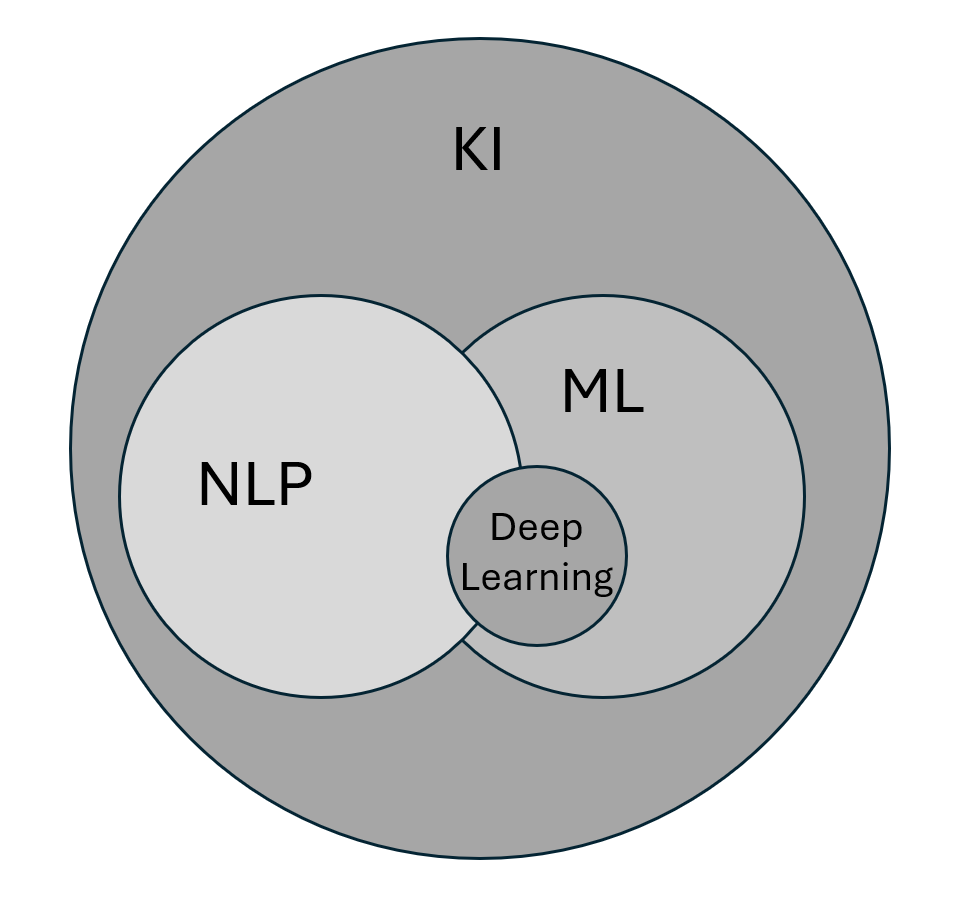
\includegraphics[width=0.6\textwidth]{img/KI_areas.png}
    \caption{Relevante Untergebiete der KI}
    \label{fig:areas_ki}
\end{figure}

Diese Technologien bilden die Grundlage für den Chatbot und ermöglichen es, Sprache zu verstehen und zu verarbeiten, um den Nutzern die gezielte und effiziente Suche nach Informationen zu erleichtern.


\section{Machine Learning und Deep Learning}

Ein wesentlicher Bestandteil der \ac{KI} ist das Machine Learning (\ac{ML}), welches es Systemen ermöglicht, Muster in großen Datenmengen zu erkennen, 
sich adaptiv zu verbessern und auf dieser Grundlage Prognosen oder Entscheidungen zu treffen. 
\ac{ML}-Modelle sind in der Lage, große Mengen an Textdaten zu verarbeiten und dabei Muster in der Sprache zu erlernen, die für die Erzeugung kohärenter und sinnvoller Antworten erforderlich sind.
Darüber hinaus ermöglicht es \ac{ML}, dass die Modelle durch kontinuierliche Interaktion mit Nutzern neue Daten aufnehmen und ihre Leistung im Laufe der Zeit optimieren. (\cite[S. 406]{Sarferaz2023})

Deep Learning ist eine spezialisierte Form des maschinellen Lernens, die auf tiefen neuronalen Netzwerken basiert. 
Diese tiefen neuronalen Netzwerke zeichnen sich durch mehrere versteckte Schichten aus, die es ermöglichen, komplexe Muster und Zusammenhänge zu erkennen. (\cite[S. 436 ff.]{LeCun2015})

In Kombination mit \ac{NLP} wird Deep Learning häufig in \ac{LLM}-Modellen eingesetzt, um tiefere semantische Strukturen und inhaltliche Verbindungen in Texten zu identifizieren. 
Durch die mehrschichtige Struktur neuronaler Netze kann Deep Learning daher die Erkennung komplexer Muster unterstützen und die Genauigkeit der vom Chatbot generierten Antworten erhöhen. (\cite[S. 605 f.]{Otter2021})


\section{Natural Language Processing}

Das Natural Language Processing (\ac{NLP}), ein spezialisiertes Teilgebiet der \ac{KI}, spielt ebenfalls eine wichtige unterstützende Rolle in dieser Arbeit. 
\ac{NLP} umfasst Techniken, die es Maschinen ermöglichen, menschliche Sprache nicht nur zu analysieren, sondern auch semantisch zu verstehen und zu generieren. (\cite[S. 31]{trapp2021})

Da der Chatbot in dieser Arbeit auf die effiziente Verarbeitung und Beantwortung von Anfragen in natürlicher Sprache ausgerichtet ist, 
unterstützt \ac{NLP} dabei, die in Dokumenten eingebetteten Informationen präzise zu extrahieren und in einer für den Nutzer verständlichen Form bereitzustellen. (\cite[S. 30]{Raj2019})

\section{Large Language Models}

Large Language Models (\acp{LLM}) sind eine Klasse von Deep Learning Modellen, die auf enorm großen Textkorpora trainiert werden, um eine Vielzahl von Sprachaufgaben zu bewältigen. 
Sie basieren in der Regel auf neuronalen Netzwerken, insbesondere auf transformatorbasierten Architekturen, die durch ihre Fähigkeit zur parallelen Verarbeitung und zur effizienten Nutzung von Kontextinformationen beeindrucken. (\cite[S. 7]{naveed2024})

Die Funktionsweise von \acp{LLM} beruht auf der Idee, dass Text als eine Sequenz von Wörtern oder Token betrachtet wird, wobei jedes Token mit dem vorherigen Kontext in Beziehung gesetzt wird (\cite[S. 4]{naveed2024}). 
Durch das Training auf Milliarden von Textbeispielen lernen die Modelle, Muster und Strukturen in der Sprache zu erkennen und basierend auf diesen Mustern Vorhersagen über die nächsten Token zu treffen. 
Je größer das Modell und je umfangreicher die Datenbasis, desto leistungsfähiger wird es in der Regel in Bezug auf das Verstehen und Generieren von Texten. (\cite[S. 1 ff.]{mielke2021})

Ein typisches \ac{LLM} ist so aufgebaut, dass es eine Vielzahl von Aufgaben wie das Verstehen von Kontext, das Beantworten von Fragen, das Verfassen von Texten oder sogar das Übersetzen von Sprachen bewältigen kann. 
Dabei greifen \acp{LLM} auf ihr internes Wissen zurück, das sie während des Trainings erworben haben, und sind in der Lage, eine Vielzahl von Aufgaben ohne spezialisierte Vorkenntnisse zu bewältigen. (\cite[S. 7]{Cerf2023})

\acp{LLM} wie GPT-4o und LLaMA3-70b basieren auf dieser Architektur und werden auf riesigen Datensätzen trainiert, die sie dazu befähigen, auf umfangreiche Sprachaufgaben zu reagieren (\cite[S. 782 f.]{Nowak2024}). 
Die in dieser Arbeit eingesetzten Modelle spielen eine zentrale Rolle, da sie die Grundlage für den Chatbot bilden, der entwickelt wird, um auf Basis von eingebetteten Dokumenten präzise und kontextbezogene Antworten zu generieren.

Ein entscheidender Vorteil von \acp{LLM} ist ihre Fähigkeit, auch komplexe Anfragen zu verstehen und im Kontext des gesamten Gesprächsverlaufes oder eines Dokumentenbestandes zu interpretieren. 
Die Verwendung von \ac{LLM} in Kombination mit \ac{RAG} verbessert zusätzlich die Fähigkeit des Chatbots, auf aktuelle und spezifische Informationen zuzugreifen (\cite[S. 1]{chen2023}). 

\section{Retrieval-Augmented Generation}

Retrieval-Augmented Generation (\ac{RAG}) ist ein fortschrittlicher Ansatz für \acp{LLM}, der für die Entwicklung von Chatbots relevant ist, die auf eingebetteten Dokumenten basieren. 
\ac{RAG} kombiniert \acp{LLM} mit einer Abrufkomponente, die es dem System ermöglicht, in Echtzeit externe Informationen aus einer Dokumentensammlung abzurufen anhanddessen eine Antwort zu generieren. 
Diese Methode erweist sich als besonders effizient, wenn präzise und aktuelle Informationen bereitgestellt werden sollen. (\cite[S. 1 ff.]{akkiraju2024factsbuildingretrievalaugmented}).

Im Rahmen dieser Arbeit wird \ac{RAG} verwendet, um sicherzustellen, dass der Chatbot nicht nur auf vortrainiertes Wissen zurückgreift, sondern auch spezifische Informationen aus eingebetteten Dokumenten bezieht. 
Dies ist besonders wichtig für die Freudenberg Gruppe, da der Chatbot auf unternehmensspezifische Dokumente zugreifen muss, um präzise Antworten zu generieren, die den Informationsbedarf der Mitarbeiter decken (\cite[S. 2]{akkiraju2024factsbuildingretrievalaugmented}).

Eine zentrale Technologie, die es dem Chatbot ermöglicht, diese Dokumente effizient zu durchsuchen und relevante Informationen zu extrahieren, ist das Embedding. 

\section{Embedding}

Embedding stellt eine grundlegende Technologie im \ac{RAG}-Prozess dar, die Wörter, Phrasen und ganze Dokumente in numerische Vektoren transformiert. 
Diese Vektoren repräsentieren semantische Beziehungen und ermöglichen es dem Chatbot, kontextuelle Zusammenhänge zwischen Textinhalten präzise zu identifizieren und relevante Informationen effizient zu extrahieren. (\cite[S. 1 ff.]{tennenholtz2024})

Wichtige Parameter im Embedding-Prozess sind die \textit{chunk size} und der \textit{top k}-Wert. Die \textit{chunk size} bezeichnet die Größe der Textabschnitte, in die ein Dokument aufgeteilt wird, 
bevor diese in Vektoren umgewandelt werden. Eine kleinere \textit{chunk size} ermöglicht eine feingranulare Analyse, während größere Chunks den Vorteil haben, umfassendere Zusammenhänge zu bewahren. 
Die Wahl der optimalen \textit{chunk size} ist entscheidend, um ein Gleichgewicht zwischen Detailgenauigkeit und Übersichtlichkeit der Informationen zu erreichen. (\cite[S. 1329 ff.]{Abdelazim2023})

Der \textit{top k}-Wert legt fest, wie viele der am höchsten bewerteten Chunks als Kontextinformationen an das \ac{LLM} weitergegeben werden (\cite{llamaindex}). Ein höherer \textit{top k}-Wert erhöht die Wahrscheinlichkeit, 
dass relevante Inhalte in den Kontext einfließen, kann jedoch die Präzision verringern, da mehr Informationen berücksichtigt werden. 
Diese Parameter tragen wesentlich dazu bei, die Effizienz und Genauigkeit des Chatbots zu optimieren, indem sie steuern, 
welche und wie viele Informationen aus den eingebetteten Dokumenten in die Antworten des Modells einfließen.

In dieser Arbeit sind Embeddings von zentraler Bedeutung, da der Chatbot die Fähigkeit benötigt, Dokumente semantisch zu analysieren und kontextbezogene Antworten auf Basis dieser Dokumente zu generieren. 
Ein Mitarbeiter der Freudenberg Gruppe kann somit neue Dokumente in das System hochladen, die der Chatbot bei zukünftigen Anfragen berücksichtigt. 
Durch die Einbettung dieser Dokumente in den Vektorraum ist der Chatbot in der Lage, die neuen Inhalte in seine Antworten zu integrieren, 
wodurch eine kontinuierliche Bereitstellung aktueller und relevanter Informationen sichergestellt wird (\cite[S. 4]{akkiraju2024factsbuildingretrievalaugmented}).

\section{Open Source}

Open Source bezeichnet Software, deren Quellcode öffentlich zugänglich ist und von jedem eingesehen, verändert und weiterverbreitet werden kann. 
Diese Offenheit ermöglicht es Entwicklern, die Software individuell anzupassen und weiterzuentwickeln, was einen hohen Grad an Flexibilität und Anpassbarkeit bietet. (\cite[S. 1]{Engelfried2010})
In bezug auf \ac{KI} bedeutet dies, dass Unternehmen \ac{LLM} nutzen können, ohne ihre Daten an externe Anbieter weitergeben zu müssen.

Für die Freudenberg Gruppe bietet die Nutzung von Open-Source-Lösungen signifikante Vorteile in Bezug auf Datenschutz und Datenhoheit. 
Durch die Implementierung in einer geschützten Umgebung wird sichergestellt, dass sensible Daten nicht an externe Anbieter wie Amazon oder Google übertragen werden müssen. 
Dies ist besonders wichtig, um strenge Datenschutzrichtlinien einzuhalten und die volle Kontrolle über die Daten zu behalten (\cite[S. 781 f.]{Nowak2024}).

Diese strategischen und technischen Überlegungen sind besonders wichtig für die Implementierung eines sicheren und datenschutzkonformen Chatbots, da sie es dem Unternehmen ermöglichen, 
sowohl die technische Infrastruktur als auch die Datensicherheit vollständig zu kontrollieren.

\section{SAP Business Technology Platform}

Die SAP Business Technology Platform (\ac{BTP}) ist eine umfassende cloudbasierte Plattform, die eine Vielzahl von Diensten bereitstellt, um Unternehmen bei der digitalen Transformation, 
Innovation und dem Wachstum zu unterstützen. Die \ac{BTP} umfasst zentrale Funktionen wie Anwendungsentwicklung, Integration, Datenmanagement, 
Analytik sowie Lösungen für Künstliche Intelligenz (\ac{KI}) und Maschinelles Lernen (\ac{ML}) (\cite[S. 103]{Gupta2024}). 

Zu den integrierten Lösungen gehören unter anderem SAP HANA, SAP Analytics Cloud, die SAP Intelligent Enterprise Suite sowie Enterprise AI. 
Diese Plattform ermöglicht es Unternehmen, ihre Geschäftsprozesse durch eine enge Integration und die Erweiterbarkeit der bereitgestellten Dienste zu optimieren und zu automatisieren. 
Die \ac{BTP} bietet sowohl vorgefertigte \ac{KI}-Anwendungen als auch die Möglichkeit, eigene, maßgeschneiderte Lösungen zu entwickeln und in die Unternehmensinfrastruktur zu integrieren. 
Mit der Einführung der \ac{BTP} im Jahr 2021, die die SAP Cloud Platform ersetzte, wurde eine intelligente Geschäftsmanagementplattform geschaffen, 
die die Kernfunktionalitäten von SAP S/4HANA umfasst und weltweite Echtzeit-Geschäftsoperationen ermöglicht. (\cite[S. 8 f.]{hrischevartificial}) 

Ein zentrales Element der \ac{BTP} ist die Cloud Foundry-Umgebung, die als Fundament der Plattform dient und eine cloudbasierte Laufzeitumgebung für die Entwicklung und Ausführung von Anwendungen bietet. 
Entwickler können hier Anwendungen in verschiedenen Programmiersprachen erstellen und bereitstellen, was der \ac{BTP} eine hohe Flexibilität verleiht. 
Die Cloud Foundry ist damit eine der Kernkomponenten der SAP \ac{BTP}, die es ermöglicht, cloud-native Anwendungen effizient zu betreiben. (\cite{sap2024cloudFoundry})

Für diese Arbeit ist die \ac{BTP} von besonderer Bedeutung, da sie die Grundlage für die Entwicklung und das Hosting des Chatbots darstellt. 
Insbesondere durch die flexible Nutzung der Cloud Foundry-Umgebung ermöglicht die \ac{BTP} es, die auf der Plattform verfügbaren \acp{LLM} effizient zu nutzen, 
um den Chatbot sicher und skalierbar in bestehende Geschäftsprozesse zu integrieren.

\section{SAP AI Core}

SAP AI Core bildet die zentrale Laufzeitumgebung für die Bereitstellung und das Management von Large Language Models (\acp{LLM}) und Embedding-Modellen auf der \ac{BTP} (\cite{sap2023aiCore}). 
Die Plattform stellt alle notwendigen Werkzeuge und eine flexible Infrastruktur bereit, um vortrainierte Modelle in produktiven Anwendungen einzusetzen und ihre Nutzung in Geschäftsprozesse zu integrieren. 
SAP AI Core ermöglicht diese Einbindung durch eine standardisierte \ac{API}-Schnittstelle, die eine direkte Integration in SAP-Anwendungen und bestehende Geschäftsanwendungen unterstützt. (\cite{sap2024aiCore})
Für die Entwicklung des Chatbots in dieser Arbeit ist SAP AI Core somit von zentraler Bedeutung, da es eine einfache Anbindung an die gewählten \acp{LLM} und die relevanten \ac{KI}-Funktionen bietet (\cite[S. 9]{hrischevartificial}).

Neben der Integration von SAP AI Core über die \ac{API}-Schnittstelle bietet SAP auch eine Python AI Core \ac{SDK}, die die Kommunikation und Interaktion mit den \acp{LLM} erheblich vereinfacht (\cite{sap2024aiCore}). 
Diese \ac{SDK} bietet leicht zugängliche Funktionen, um Prompts zu senden und Antworten zu empfangen, 
was die Implementierung von Retrieval-Augmented Generation (\ac{RAG}) in den Chatbot unterstützt und die Nutzung vortrainierter Modelle optimiert. 
So kann der Chatbot der Freudenberg Gruppe die benötigten Informationen auf Grundlage der eingebetteten Dokumente effizient bereitstellen, ohne die Notwendigkeit zusätzlicher Modelltrainings. (\cite{pythonAICoreSDK})

Mit SAP AI Core profitieren Anwender von einer verwalteten Umgebung, die alle notwendigen Abhängigkeiten integriert und somit den Aufwand für den Aufbau einer eigenen Modellinfrastruktur reduziert (\cite{sap2024aiCore}).
Dies schafft eine zuverlässige und einfach zu handhabende Umgebung für produktive \ac{KI}-Anwendungen und trägt dazu bei, \ac{KI}-Projekte schneller und kosteneffizienter in die Realität umzusetzen.

\section{LlamaIndex}

LlamaIndex ist eine zentrale Komponente zur Implementierung von Retrieval-Augmented Generation (\ac{RAG}) in Chatbots. 
Es ermöglicht eine effiziente semantische Suche innerhalb großer Dokumentbestände und erlaubt dem Chatbot, relevante Informationen in Echtzeit abzurufen und diese in die Antwortgenerierung zu integrieren (\cite{llamaindex}).

In der vorliegenden Arbeit wird LlamaIndex zur Entwicklung des Chatbots genutzt, indem es eine eine Similarity-Suche zwischen Benutzeranfragen und den eingebetteten Dokumenten durchführt und somit relevante Abschnitte identifiziert. 
Dies steigert die Relevanz und Genauigkeit der generierten Antworten und ermöglicht es den Mitarbeitern der Freudenberg Gruppe, schnell und präzise auf die benötigten Informationen zuzugreifen.
\cleardoublepage

\chapter{Analyse und Konzept}
\label{analyse}
\nocite{*}

In diesem Kapitel wird zunächst eine allgemeine Analyse der gruppenweiten Anwendungsfälle für Künstliche Intelligenz (\ac{KI}) innerhalb der Freudenberg Gruppe durchgeführt. 
Darauf aufbauend wird der Fokus auf die spezifische Entwicklung eines Chatbots gerichtet, indem relevante Anwendungsfälle und die potenziellen Mehrwerte eines solchen Systems im Unternehmenskontext analysiert werden.

Auf Basis der gewonnenen Erkenntnisse wird ein Konzept zur systematischen Untersuchung von Large Language Models (\acp{LLM}) und Embedding-Modellen erstellt. 
Dieses Konzept dient als Grundlage für die technische Implementierung und die fundierte Auswahl geeigneter Modelle zur optimalen Unterstützung der definierten Anwendungsfälle.

\section{Analyse der Anwendungsfälle}
\subsection{Gruppenweite Anwendungsfälle}

Die Freudenberg Gruppe bietet mit ihren vielfältigen Geschäftsbereichen ein breites Einsatzspektrum für \ac{KI}-Technologien. 
Jede Geschäftseinheit hat spezifische Anforderungen und Herausforderungen, die durch den Einsatz von Künstlicher Intelligenz adressiert werden können. 
So nutzt beispielsweise Freudenberg Sealing Technologies \ac{KI}-basierte Lösungen zur automatischen Sichtkontrolle in der Produktion, um Defekte frühzeitig zu erkennen und zu beheben (\cite{FST_Magazin_KI}). 
Freudenberg Home and Cleaning Solutions setzt \ac{KI} zur Optimierung von Spritzgießmaschinen ein, indem Produktionsdaten analysiert und Optimierungsvorschläge generiert werden, 
was sowohl die Maschinenleistung als auch die Produktqualität verbessert (\cite{Spritzgießen_4.0}).

Trotz der vielfältigen Einsatzmöglichkeiten von \ac{KI} in den Produktionsprozessen gibt es bisher jedoch keinen gruppenweiten Einsatz eines \ac{KI}-basierten Chatbots. 
Ein solcher Chatbot sollte die internen Kommunikationsprozesse erheblich optimieren, indem er Routineanfragen automatisiert und den Zugriff auf wichtige Informationen erleichtert. 
In der aktuellen Phase der digitalen Transformation ist die Einführung eines Chatbots besonders relevant, um die Effizienz in der Informationsbeschaffung zu steigern und gruppenweite Synergien zu schaffen. 
Dieses Projekt bietet daher die Möglichkeit, durch die Implementierung eines \ac{KI}-basierten Chatbots einen Mehrwert für die gesamte Freudenberg Gruppe zu generieren.

\subsection{Relevanz für Freudenberg \& Co. KG}

Während die Freudenberg Gruppe in verschiedenen Geschäftsbereichen bereits \ac{KI}-Technologien zur Optimierung von Produktionsprozessen einsetzt, 
besteht im Bereich der internen Unternehmenskommunikation noch erhebliches Potenzial für Automatisierung und Effizienzsteigerung. 
Insbesondere Freudenberg \& Co. KG (\ac{FCO}) steht als zentrale Verwaltungseinheit vor der Herausforderung, umfangreiche interne Anfragen zu verwalten, 
die durch einen \ac{KI}-basierten Chatbot automatisiert und effizienter bearbeitet werden könnten.

Die Corporate IT (\ac{CIT}) bei \ac{FCO} übernimmt die Aufgabe, technologische Lösungen für interne Prozesse bereitzustellen, die gruppenweit eingesetzt werden können. 
Die Einführung eines \ac{KI}-basierten Chatbots würde die Effizienz bei der Bearbeitung von Standardanfragen erheblich steigern, 
indem sie zeitraubende Routineaufgaben wie Informationsrecherche und Dokumentenverwaltung automatisiert. 
Dadurch könnten \ac{CIT}-Mitarbeitende, die bisher einen Großteil ihrer Zeit auf wiederkehrende Anfragen und einfache IT-Support-Tickets verwendet haben, 
ihre Kapazitäten vermehrt auf komplexere Aufgaben wie Systemoptimierungen, Sicherheitsanalysen oder innovative Projekte konzentrieren. 
Da \ac{CIT} als zentrale Schnittstelle zwischen verschiedenen Abteilungen fungiert, 
unterstützt der Chatbot eine gruppenweit einheitliche Lösung für häufige Anfragen und trägt maßgeblich zur Beschleunigung der digitalen Transformation des Unternehmens bei.

Darüber hinaus ist es für die \ac{CIT} sinnvoll, die neue Technologie zunächst innerhalb von \ac{FCO} zu testen und Feedback von den Nutzern zu sammeln, bevor die Software gruppenweit eingeführt wird. 
Diese schrittweise Implementierung stellt sicher, dass potenzielle Probleme frühzeitig identifiziert und behoben werden können, was die Qualität und Akzeptanz des Chatbots erhöht, 
wenn er später auf größere Unternehmensbereiche ausgeweitet wird.

\subsection{Identifikation geeigneter Anwendungsfälle für einen Chatbot}

Die Implementierung eines \ac{KI}-basierten Chatbots ist besonders relevant für Bereiche wie den Einkauf, die Personalabteilung oder die IT-Sicherheit bei \ac{FCO}, 
da in diesen Abteilungen regelmäßig Anfragen zu standardisierten Prozessen und Dokumentenbearbeitungen gestellt werden. 
Ein interner Chatbot soll dazu beitragen, solche Anfragen effizient zu beantworten und gleichzeitig sicherzustellen, dass sensible Daten nach den geltenden Datenschutzbestimmungen verarbeitet werden.

Moderne \ac{KI}-Technologien wie ChatGPT oder Microsoft CoPilot haben bereits bewiesen, dass sie benutzerdefinierte Informationen in Echtzeit bereitstellen und auf komplexe Anfragen effizient reagieren können. 
Der Einsatz solcher extern gehosteten Lösungen birgt jedoch erhebliche Datenschutzrisiken, da Unternehmensdaten beim Austausch mit Dritten verarbeitet werden, 
was zu potenziellen Verstößen gegen firmeninterne Datenschutzrichtlinien führen kann. 
Um diese Risiken zu vermeiden, setzt die Freudenberg Gruppe auf die Entwicklung eines internen, auf Open-Source-Technologien basierenden Chatbots. 
Durch die Nutzung einer internen Infrastruktur bleibt die Verarbeitung sensibler Daten innerhalb der firmeneigenen IT-Umgebung, wodurch die Sicherheit und Kontrolle über die Daten gewährleistet ist. 
Darüber hinaus verbessert der interne Chatbot die Effizienz der internen Prozesse, indem er Routineanfragen eigenständig bearbeiten und relevante Informationen sofort bereitstellen kann, 
was wiederum die zeitliche Entlastung der Mitarbeiter und eine schnellere Informationsbeschaffung unterstützt.

Technologisch gesehen bietet die Nutzung von SAP AI Core in einem Subaccount der \ac{BTP} eine skalierbare und sichere Plattform für die Implementierung des Chatbots. 
Die Auswahl geeigneter \acp{LLM} und Embedding-Modelle ist dabei von entscheidender Bedeutung, um eine möglichst präzise und zuverlässige Beantwortung von Anfragen zu gewährleisten. 
Diese Modelle ermöglichen es dem Chatbot, aus großen Datenmengen zu lernen und spezifische Informationen in Echtzeit zu verarbeiten, was für die effiziente Nutzung innerhalb von \ac{FCO} von zentraler Bedeutung ist.

\section{Analyse der verfügbaren Modelle auf der BTP}
\subsection{Bewertungskriterien für die Modelle}

Die SAP \ac{BTP} bietet eine Vielzahl von Modellen für die Implementierung. Ein wesentlicher Vorteil von AI Core ist die Möglichkeit, das Large Language Model (\ac{LLM}) zur Laufzeit auszutauschen, da SAP diese Ebene abstrahiert (\cite{sap2024aiCore}). 
Dies gewährleistet, dass bei der Modellauswahl keine langfristigen Einschränkungen berücksichtigt werden müssen. Sollte ein verbessertes Modell verfügbar werden, kann es jederzeit implementiert werden.

Die Auswahl der Modelle erfolgt unter Berücksichtigung verschiedener Kriterien wie Open-Source-Lizenzierung, Antwortgeschwindigkeit, Antwortqualität und Kosten. 
Insbesondere spielt die Sicherheit eine entscheidende Rolle, besonders wenn es darum geht, firmeninterne sensible Daten zu verarbeiten. 

Dies unterstreicht die Bedeutung der \ac{BTP} als idealen Ort für die Implementierung von \ac{LLM}-basierten Lösungen. 
Im Vergleich zu Plattformen wie Microsoft Azure, die zwar ebenfalls die Entwicklung von Chatbots mit Embedding-Modellen ermöglichen, bietet die \ac{BTP} die Flexibilität, aus einer breiten Palette von Modellen zu wählen, 
ohne die Kontrolle über firmeninterne Daten zu gefährden.

\subsection{Untersuchungskonzept von Large Language Modellen}
\label{eval_llm_konzept}

Zur Prüfung der zuvor definierten Kriterien Open-Source-Lizenzierung, Antwortgeschwindigkeit, Antwortqualität und Kosten wird ein umfassendes Untersuchungskonzept für \acp{LLM} entwickelt. 
Die Bewertung der Antwortqualität erfolgt durch die Erstellung eines Datensatzes aus jeweils 10 deutschen und 10 englischen Dokumenten. 
Für diese Dokumente werden insgesamt 100 Prompts mit entsprechenden perfekten Antworten erstellt.

Die Prompts werden im ersten Schritt mit verschiedenen Einstellungen bezüglich \textit{chunk size} und \textit{top k} an verschiedene Large Language Models (\acp{LLM}) gesendet. 
Der Parameter \textit{chunk size} definiert die Größe der Textabschnitte (Chunks), in die das Dokument aufgeteilt wird, bevor es verarbeitet wird. 
Ein größerer \textit{chunk size}-Wert führt zu längeren Textabschnitten, die als Einheit betrachtet werden. Der Parameter \textit{top k} bestimmt die Anzahl der höchsten bewerteten Antworten, die das Modell als Kontextinformation zum Prompt erhält. 
Ein höherer \textit{top k}-Wert erhöht die Informationen, die das \ac{LLM} erhält, kann aber auch die Relevanz verringern.

Im zweiten Schritt werden die erhaltenen Antworten zusammen mit den erwarteten perfekten Antworten an GPT-3.5-Turbo geschickt, um einen Ähnlichkeitsscore zwischen 0 und 10 zu erhalten. 
Der Durchschnitt dieser Scores über alle Prompts ergibt das Gesamtergebnis einer Konfiguration. 
Zusätzlich werden die Laufzeit und die verbrauchten Tokens gemessen, um auf Basis der Preisstruktur von SAP AI Core auch die Kosten in die Bewertung einfließen zu lassen.

Die Antwortgeschwindigkeit wird durch die Messung der Zeit, die jedes Modell benötigt, um eine Antwort zu generieren, bewertet. Dies ermöglicht eine direkte Vergleichbarkeit der Effizienz der verschiedenen Modelle.

Auf Basis der gemessenen Werte für Antwortqualität, Antwortgeschwindigkeit und Kosten wird eine Score Function entwickelt, die eine ganzheitliche Bewertung der Modelle ermöglicht. 
Dabei wird die Antwortqualität als das wichtigste Kriterium festgelegt und mit einem Gewicht von 10 versehen. Um die Gewichtungen für Antwortgeschwindigkeit und Kosten festzulegen, 
wird eine interne Umfrage unter den Testnutzern durchgeführt. Den Teilnehmern der Umfrage wird die Möglichkeit gegeben, die Bedeutung von Geschwindigkeit und Kosten auf einer Skala von 1 bis 5 zu bewerten. 
Dies stellt sicher, dass Qualität das wichtigste Kriterium bleibt, während Geschwindigkeit und Kosten entsprechend der Nutzerpräferenzen gewichtet werden. 
Ziel ist es, durch diese Gewichtung eine realistische Abbildung der Anforderungen an den Chatbot zu gewährleisten.

\subsection{Konzept zur Untersuchung von Embedding Modellen}
\label{eval_embedding_konzept}

Die Untersuchung von Embedding-Modellen ist von zentraler Bedeutung, um ihre Leistungsfähigkeit hinsichtlich der semantischen Suche und des Auffindens relevanter Informationen in großen Dokumentensammlungen zu bewerten. 
Ziel der Untersuchung ist es, zu prüfen, wie präzise die Modelle relevante Textstellen identifizieren und korrekt in eine Rangfolge einordnen.

Für die Untersuchung werden umfangreiche Dokumente verwendet, die in kleinere Abschnitte (Chunks) unterteilt werden. 
Diese Dokumente, die eine Mischung aus technischen Berichten und allgemeinen Texten wie Wikipedia-Artikeln umfassen, wurden speziell aufgrund ihrer Größe ausgewählt, 
um die Modelle auf ihre Fähigkeit zur Verarbeitung umfangreicher Informationen zu testen. Definierte Prompts, die spezifische Textstellen in diesen Dokumenten referenzieren, werden in die Modelle eingespeist. 
Anschließend wird geprüft, ob und in welcher Rangfolge die relevanten Textabschnitte gefunden werden. Hierbei wird ein sehr hoher \textit{top k}-Wert gewählt, 
um eine möglichst breite Erfassung der relevanten Informationen zu gewährleisten und die Präzision der Modelle über mehrere Positionen hinweg zu analysieren.

Die Leistungsbewertung der Embedding-Modelle erfolgt anhand des \ac{MRR}, der misst, wie hoch die korrekte Antwort in der Ergebnisliste platziert wird. Ein hoher \ac{MRR}-Wert deutet darauf hin, 
dass das Modell in der Lage ist, die relevanten Textstellen präzise zu ordnen. 
Zusätzlich wird die Genauigkeit der Top-Ergebnisse durch die Metrik \textit{Precision at k} bewertet, welche angibt, wie viele der zurückgegebenen Ergebnisse tatsächlich relevant sind. 
Diese Metriken sind entscheidend, um die Qualität der semantischen Suche der Modelle objektiv zu beurteilen.

Neben der inhaltlichen Präzision wird auch die Performanz der Modelle hinsichtlich der Antwortgeschwindigkeit und des Ressourcenverbrauchs untersucht. 

Durch diese Untersuchung wird eine fundierte Entscheidungsgrundlage geschaffen, um das am besten geeignete Embedding-Modell für den internen Chatbot bei Freudenberg auszuwählen. Das Modell muss in der Lage sein, 
große Dokumentensammlungen effizient zu durchsuchen und relevante Informationen präzise zurückzugeben, um die Nutzer in ihrer Arbeit bestmöglich zu unterstützen.

\cleardoublepage

\chapter{Evaluation}
\label{evaluation}
\nocite{*}

In diesem Kapitel werden die Ergebnisse der Untersuchung der Large Language Models (\acp{LLM}) und Embedding-Modelle umfassend dargestellt und ausgewertet. 

Die Ergebnisse dieser Untersuchung bilden die Grundlage für die abschließende Entscheidung zur Auswahl der geeigneten Modelle und dienen als Referenz für die technische Umsetzung im nachfolgenden Abschnitt.

\section{Evaluation Large Language Modellen}
\label{eval_llm}

Im Rahmen der Entwicklung eines \ac{KI}-basierten Chatbots für Freudenberg \& Co. KG (\ac{FCO}) wurde, basierend auf dem in Abschnitt \ref{eval_llm_konzept} vorgestellten Untersuchungskonzept, 
eine umfassende Untersuchung verschiedener Large Language Models (\acp{LLM}) durchgeführt, die auf SAP AI Core innerhalb der SAP Business Technology Platform (\ac{BTP}) verfügbar sind. 
Da diese Modelle für die geplante Implementierung des Chatbots relevant sind, konzentriert sich die Untersuchung auf die in SAP AI Core angebotenen Modelle, 
um eine fundierte Entscheidung für die spezifischen Anforderungen des Projekts treffen zu können.

Die getesteten Modelle umfassen die Open-Source-Modelle \textit{LLaMA3-70b}, \textit{Mistral-8x7b}, \textit{Falcon-40b} sowie die Modelle \textit{GPT-3.5-Turbo} und \textit{GPT-4o} von OpenAI. 
Jedes Modell wurde unter verschiedenen Konfigurationen evaluiert, wobei \textit{chunk sizes} von 64, 128, 256 und 512 getestet wurden. Zudem wurden die \textit{top k}-Werte 4, 6, 8, 10, 15 und 20 verwendet, 
um die Anzahl der in den Kontext einbezogenen Antworten zu variieren. Dies führte insgesamt zu 24 Konfigurationen pro Modell, was eine umfassende und detaillierte Bewertung der Leistungsfähigkeit ermöglicht.

Für jede Konfiguration wurden 100 Prompts durchgeführt, die auf 10 deutsche und 10 englische Dokumente verteilt waren. Die Ergebnisse für jedes \ac{LLM} wurden gespeichert, 
um eine genaue Analyse der Leistung unter den verschiedenen Konfigurationen zu ermöglichen. Anschließend wurde der Durchschnitt der Ergebnisse pro Konfiguration und Modell berechnet, 
um eine Vergleichbarkeit zu gewährleisten und präzise Aussagen darüber treffen zu können, wie die einzelnen \acp{LLM} bei jeder Konfiguration performen.

Die Vielzahl der getesteten Parameter gewährleistet, dass die Modelle auf einer breiten Datenbasis evaluiert werden, um präzise Rückschlüsse auf ihre Leistungsfähigkeit zu ziehen. 
Darüber hinaus hilft diese Untersuchung dabei, die optimalen Parameterkonfigurationen für den praktischen Einsatz im Chatbot zu bestimmen.

Die Evaluation erfolgt unter Berücksichtigung der Kriterien Antwortqualität, Antwortzeit und Kosten. Diese Kriterien stellen sicher, dass das ausgewählte Modell nicht nur qualitativ hochwertige und relevante Antworten liefert, 
sondern auch effizient und kostengünstig in Echtzeitanwendungen integriert werden kann.

In den folgenden Abschnitten werden die Ergebnisse der Evaluation detailliert analysiert und die Leistung der Modelle miteinander verglichen.

\subsection{Antwortqualität}

Die Antwortqualität der verschiedenen \acp{LLM} wurde anhand einer normalisierten Bewertungsfunktion \ref{eq:score_function_quali} ermittelt. 
Hierbei wurde der Ähnlichkeitsscore, den \textit{GPT-3.5-Turbo} für jede generierte Antwort in Bezug auf eine perfekte Antwort vergeben hat, 
auf eine Skala von 0 bis 1 normalisiert und anschließend mit einem Faktor von 10 multipliziert. 
Dies ermöglicht eine einheitliche Bewertung der Antwortqualität auf einer Skala von 0 bis 10, wobei 10 die höchste Übereinstimmung mit der perfekten Antwort darstellt.

Diese Normalisierung stellt sicher, dass die Bewertung der Antwortqualität für alle Modelle konsistent und vergleichbar bleibt. 
Sie minimiert Verzerrungen und garantiert, dass die Modelle im Verhältnis zu ihrer maximal erreichbaren Leistung bewertet werden.

\begin{equation}
    \mbox{Score Function} = \mbox{gpt-3.5-turbo\_judgement} \cdot 10
    \label{eq:score_function_quali}
\end{equation}

In Abbildung \ref{fig:antwortqualität} sind die Ergebnisse der Antwortqualität in Form eines Streudiagramms dargestellt. 
Auf der X-Achse sind die unterschiedlichen Konfigurationen von \textit{chunk size} und \textit{top k} abgetragen, während die Y-Achse den Antwort-Score von 0 bis 10 wiedergibt.
Die Modelle \textit{GPT-4o}, \textit{GPT-3.5-Turbo} und \textit{LLaMA3-70b} erreichen konsistent hohe Scores, was ihre Fähigkeit zur präzisen und relevanten Beantwortung komplexer Anfragen unterstreicht.
\textit{GPT-4o} zeigt hierbei in den meisten Konfigurationen die höchsten Scores, was seine besondere Eignung für die präzise Bearbeitung anspruchsvoller Anfragen hervorhebt.
Im Gegensatz dazu erzielt \textit{Falcon-40b} durchgehend niedrigere Scores, was auf eine geringere semantische Präzision und Genauigkeit seiner Antworten schließen lässt.

\begin{figure}[H]
    \centering
    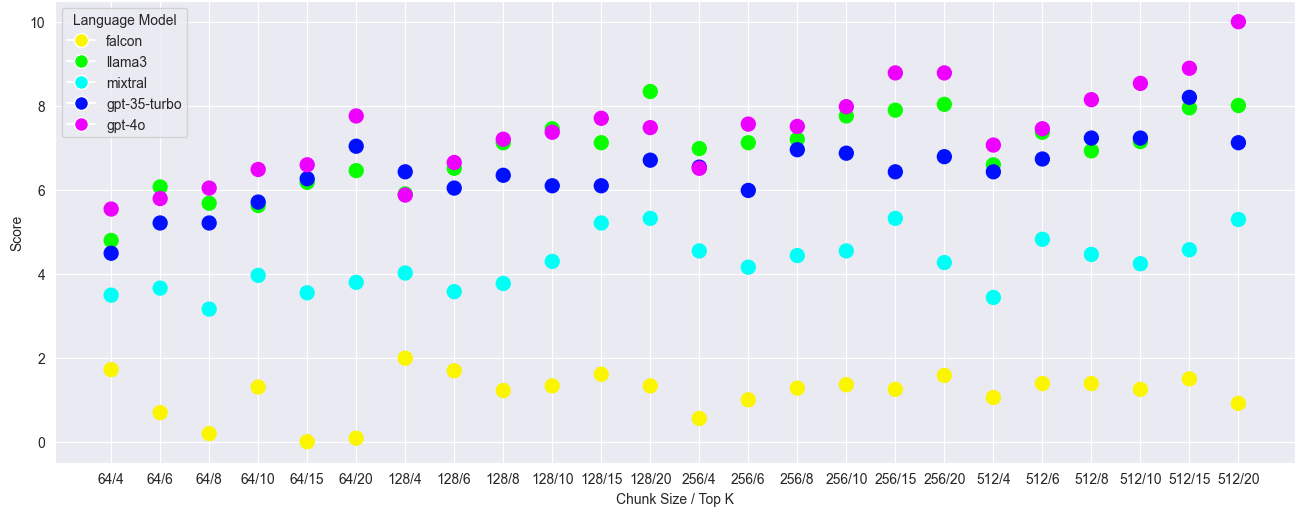
\includegraphics[width=1\textwidth]{img/antwortquali.png}
    \caption{Antwortqualität Untersuchung \acp{LLM}}
    \label{fig:antwortqualität}
\end{figure}

\subsection{Antwortzeit}

Die Antwortzeit stellt ein zentrales Kriterium für die Praktikabilität von \acp{LLM} in Echtzeitanwendungen dar. Um diese zu bewerten, wurde die Laufzeit für jede Anfrage gemessen, beginnend mit dem Zeitpunkt des Absendens eines Prompts bis zur Rückgabe der Antwort durch das Modell.
Anschließend wurde für jede Konfiguration der Durchschnitt der Laufzeiten berechnet.

Das berechnete Ergebnis wird in der Bewertungsfunktion \ref{eq:score_function_zeit} als Maß für die Effizienz der jeweiligen Konfiguration verwendet.

\begin{equation}
    \mbox{Score Function} = \mbox{avg\_runtime}
    \label{eq:score_function_zeit}
\end{equation}

Alle Tests wurden unter denselben Bedingungen in einem stabilen lokalen LAN-Netzwerk auf identischer Hardware durchgeführt. 
Diese kontrollierte Umgebung stellte sicher, dass die Laufzeiten der Modelle unter fairen und vergleichbaren Bedingungen ermittelt wurden.

In Abbildung \ref{fig:antwortzeit} sind die durchschnittlichen Antwortzeiten der Modelle als Streudiagramm dargestellt. 
Auf der X-Achse sind die unterschiedlichen Konfigurationen von \textit{chunk size} und \textit{top k} dargestellt, während die Y-Achse die Antwortzeit (Runtime) in Millisekunden wiedergibt. 
Die Werte reichen hierbei von unter 1000 ms bis knapp unter 9000 ms.
Modelle wie \textit{GPT-4o} und \textit{GPT-3.5-Turbo} verzeichneten durchweg kurze Antwortzeiten, was sie besonders für den Einsatz in Echtzeitanwendungen prädestiniert. 
Im Gegensatz dazu zeigte das Modell \textit{Falcon-40b} signifikant längere Antwortzeiten, was dessen Einsatzpotenzial in zeitkritischen Szenarien deutlich einschränkt.

Die Unterschiede in der Antwortzeit lassen sich teilweise auf die Infrastrukturen zurückführen, die hinter den Modellen stehen. 
Modelle von OpenAI, wie \textit{GPT-4o} und \textit{GPT-3.5-Turbo}, profitieren von spezialisierter Hardware in hoch optimierten Rechenzentren, was ihre Geschwindigkeit verbessert. 
Open-Source-Modelle wie \textit{Falcon-40b} haben oft nicht denselben Zugang zu spezialisierten Infrastrukturen, was sich negativ auf ihre Laufzeiten auswirkt.

\begin{figure}[H]
    \centering
    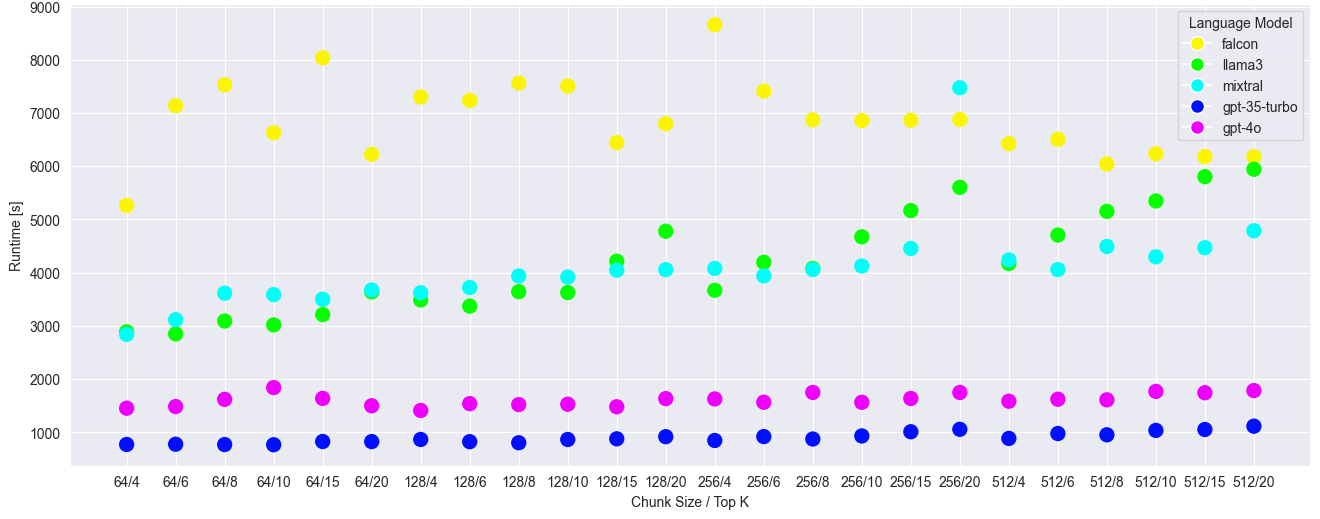
\includegraphics[width=1\textwidth]{img/antwortzeit.png}
    \caption{Antwortzeiten Untersuchung \acp{LLM}}
    \label{fig:antwortzeit}
\end{figure}

\subsection{Kosten}

Die Kostenbewertung der Large Language Models (\acp{LLM}) basiert auf der Messung des Tokenverbrauchs pro Anfrage. 
Der Tokenverbrauch wurde bei jedem Untersuchungslauf gemessen, wobei für einige Modelle, wie \textit{GPT-4o} und \textit{GPT-3.5-Turbo}, der Tokenverbrauch direkt von den \acp{API} von SAP AI Core bereitgestellt wird. 
Für Modelle, die diese Information nicht nativ liefern, wie \textit{LLaMA3-70b}, wurde die Token-Anzahl mithilfe der Python-Library \textit{tokenizers} ermittelt. 
Dieses Tool ermöglicht eine präzise Berechnung des Tokenverbrauchs anhand der jeweiligen Tokenizer-Spezifikationen der Modelle. 
Die \textit{tokenizer.json}-Dateien für die entsprechenden Modelle wurden dabei von der Plattform Hugging Face heruntergeladen und verarbeitet.

Um die Gesamtkosten zu ermitteln, wurde der Tokenverbrauch für jeden Untersuchungslauf gemessen und mit den festgelegten Kosten für Input- und Output-Tokens der \acp{LLM}, wie sie von SAP AI Core vorgegeben sind, multipliziert. Um die Ergebnisse zu standardisieren, 
wurde in der Bewertungsfunktion \ref{eq:score_function_kosten} der normalisierte Durchschnitt mit einem Faktor von 10 multipliziert.

\begin{equation}
    \mbox{Score Function} = \mbox{avg\_cost} \cdot 10
    \label{eq:score_function_kosten}
\end{equation}

In Abbildung \ref{fig:kosten} sind die normalisierten Kosten pro Prompt für jede Konfiguration und jedes \ac{LLM} dargestellt. 
Die X-Achse zeigt die verschiedenen Konfigurationen hinsichtlich \textit{chunk size} und \textit{top k}, während die Y-Achse den Score von 0 bis 10 wiedergibt, wobei höhere Scores höhere Kosten anzeigen.

Die Ergebnisse verdeutlichen, dass \textit{GPT-4o} in allen Konfigurationen die höchsten Kosten verursacht, was auf den erhöhten Rechenaufwand und die Ressourcenanforderungen hinweist, 
die zur Generierung präziser und detaillierter Antworten benötigt werden. Im Gegensatz dazu sind die Kosten für \textit{Falcon-40b} und \textit{Mistral-8x7b} deutlich geringer, 
was diese Modelle insbesondere für kostensensitive Anwendungen interessant macht.



\begin{figure}[H]
    \centering
    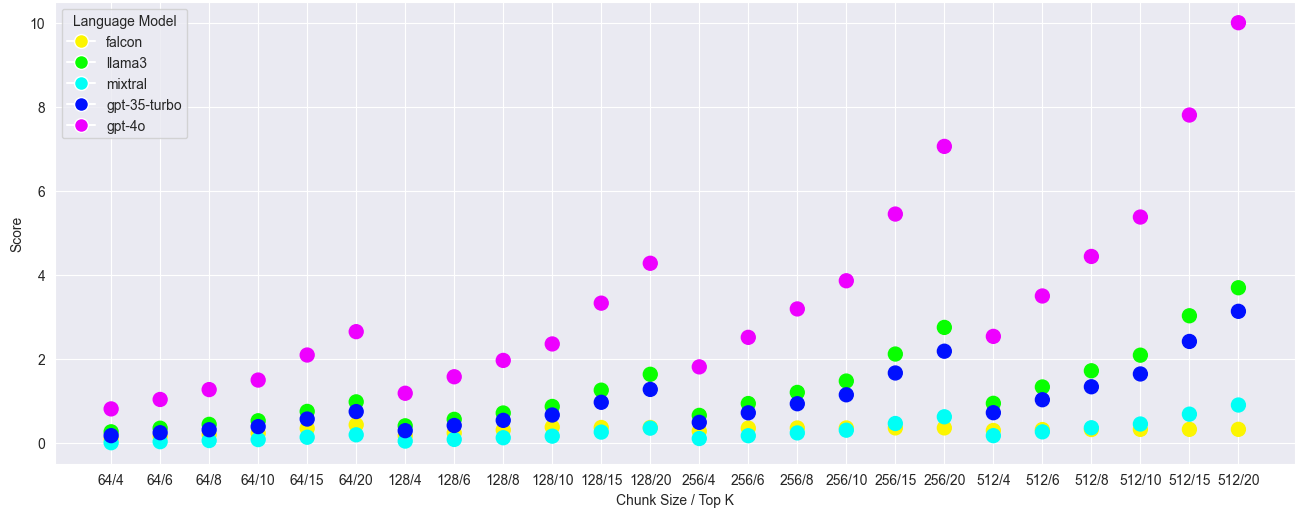
\includegraphics[width=1\textwidth]{img/kosten.png}
    \caption{Kosten Untersuchung \acp{LLM}}
    \label{fig:kosten}
\end{figure}

\subsection{Gesamtbewertung}

Die Gesamtbewertungsfunktion \ref{eq:score_function_gesamt} berücksichtigt drei Hauptkomponenten: die Qualität der Antworten, die Antwortzeit und die Gesamtkosten. 
Diese Faktoren werden mit unterschiedlichen Gewichtungen kombiniert, um eine umfassende Bewertung der Leistungsfähigkeit der Modelle zu ermöglichen.

\begin{equation}
    \mbox{Score Function} = \mbox{\textit{gpt\_judgement}} \cdot 10 - \mbox{\textit{avg\_runtime}} \cdot 2 - \mbox{\textit{total\_cost}} \cdot 5
    \label{eq:score_function_gesamt}
\end{equation}

Die \textit{gpt judgement}-Komponente bezieht sich auf die Bewertung der Antwortqualität, die durch \textit{GPT-3.5-Turbo} vorgenommen wurde. 
Die Antwortqualität wurde auf einer Skala von 0 bis 1 normalisiert und anschließend mit 10 multipliziert, um sie in den gleichen Wertebereich wie die anderen Faktoren zu skalieren. 
Die \textit{average runtime} wurde ebenfalls auf einer Skala von 0 bis 1 normalisiert, um sicherzustellen, dass die Laufzeitfaktoren vergleichbar verrechnet werden können. 
Die \textit{total cost}-Komponente umfasst die Gesamtkosten, die mit jedem Prompt verbunden sind, und wurde ebenfalls auf einer Skala von 0 bis 1 normalisiert, 
um die finanzielle Effizienz der Modelle in Bezug auf deren Leistungsfähigkeit zu bewerten.

Die Gewichtung der Antwortzeit mit dem Faktor 2 und der Kosten mit dem Faktor 5 in der Score Function \ref{eq:score_function_gesamt} basiert auf den Ergebnissen einer internen Umfrage unter Testnutzern, 
wie im Untersuchungskonzept \ref{eval_llm_konzept} beschrieben. Diese Umfrage erfasste die Prioritäten der Testnutzer hinsichtlich Antwortgeschwindigkeit und Kosten, 
während die Antwortqualität als das wichtigste Kriterium festgelegt und mit einem Faktor von 10 gewichtet wurde.

Leider trat während der Sicherung der Umfrageergebnisse ein Fehler im Backup-Prozess auf, der dazu führte, dass die Rohdaten irreversibel verloren gingen. 
Jedoch wurden die Umfrageergebnisse zuvor in einer Excel-Datei gesichert, was die Berechnung von Mittelwert und Median ermöglichte, sodass diese Kennzahlen weiterhin zur Verfügung stehen.

In Abbildung \ref{fig:prioritäten} sind die Antworten der Umfrage visualisiert. 
Für die Antwortgeschwindigkeit ergab sich ein Mittelwert von 2,09 und ein Median von 2, was darauf hindeutet, dass Geschwindigkeit als relevant, aber nicht als primäres Kriterium angesehen wird. 
Im Gegensatz dazu zeigt das Ergebnis für die Kosten einen Mittelwert von 4,55 und einen Median von 5, was die hohe Bedeutung der Kosten für die Testnutzer verdeutlicht.

\begin{figure}[H]
    \centering
    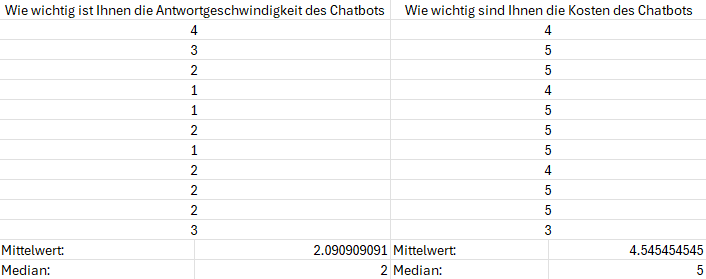
\includegraphics[width=0.8\textwidth]{img/prioritaeten.png}
    \caption{Prioritäten der Testnutzer in Bezug auf Antwortgeschwindigkeit und Kosten}
    \label{fig:prioritäten}
\end{figure}

Diese Umfrageergebnisse wurden herangezogen, um die Gewichtungen der \textit{avg runtime} und \textit{total cost} in der Score Function \ref{eq:score_function_gesamt} zu bestimmen. 
Dadurch wird gewährleistet, dass Modelle, die qualitativ hochwertige Antworten liefern, gleichzeitig effizient in der Laufzeit und kostengünstig sind, 
die höchste Gesamtbewertung erzielen. Die Score Function ermöglicht somit eine ausgewogene Berücksichtigung aller relevanten Faktoren und unterstützt eine fundierte Entscheidungsfindung bei der Auswahl der geeignetsten Modelle.

In Abbildung \ref{fig:gesamtwert} sind die Ergebnisse der Gesamtbewertung der Modelle dargestellt. 
Die Modelle \textit{GPT-4o}, \textit{GPT-3.5-Turbo} und \textit{LLaMA3-70b} erreichten hierbei die höchsten Scores, was auf ihre gute Balance zwischen Antwortqualität, Antwortzeit und Kosten hinweist. 
\textit{Falcon-40b} hingegen erzielte aufgrund seiner geringeren Antwortqualität und längeren Antwortzeiten eine vergleichsweise niedrige Gesamtbewertung.

\begin{figure}[H]
    \centering
    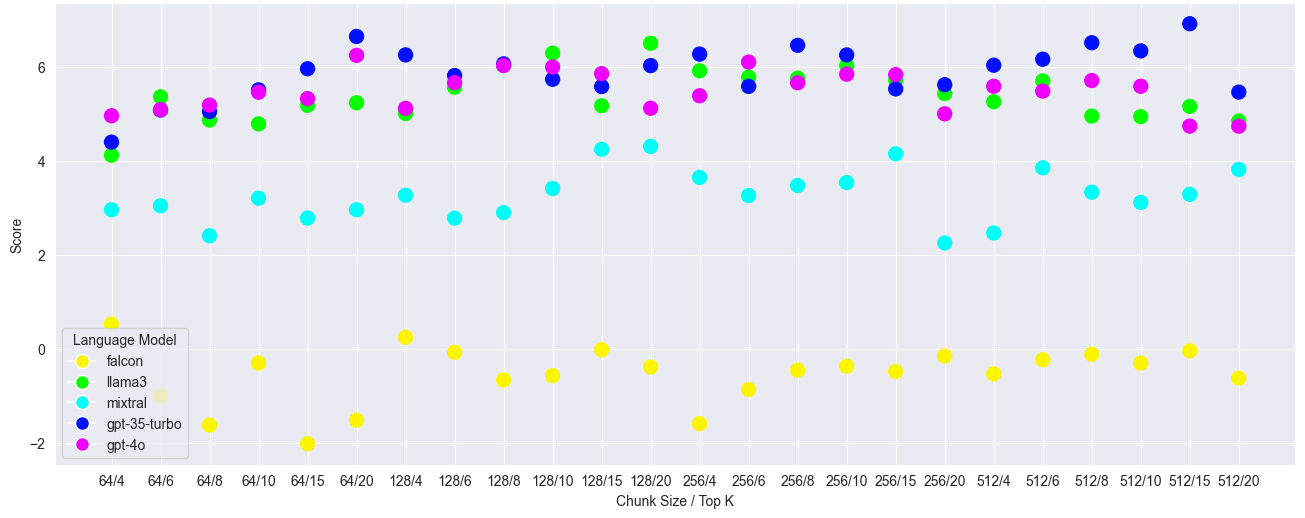
\includegraphics[width=1\textwidth]{img/gesamtScore.png}
    \caption{Gesamtbewertung der Untersuchung der \acp{LLM}}
    \label{fig:gesamtwert}
\end{figure}

Auf Basis dieser Ergebnisse lässt sich festhalten, dass \textit{LLaMA3-70b} das beste Open-Source-Modell darstellt, während \textit{GPT-3.5-Turbo} in der Gesamtbewertung die besten Leistungen erbringt. 
Sollte in der Score Function \ref{eq:score_function_gesamt} die Gewichtung der Kosten reduziert oder entfernt werden, wäre \textit{GPT-4o} das leistungsstärkste Modell.

Die Ergebnisse dieser Evaluation bieten eine solide Grundlage für die Auswahl der am besten geeigneten Modelle, um den spezifischen Anforderungen der Freudenberg Gruppe gerecht zu werden. 
Wenn Open-Source-Anforderungen bestehen, ist \textit{LLaMA3-70b} die beste Wahl. Sollte das Budget keine Rolle spielen, empfiehlt sich \textit{GPT-4o}. 
Andernfalls stellt \textit{GPT-3.5-Turbo} die effizienteste Option dar.

\section{Evaluation von Embedding Modellen}
\label{eval_embedding}

Die Untersuchung der Embedding-Modelle basiert auf dem in Abschnitt \ref{eval_embedding_konzept} beschriebenen Konzept. Ziel der Evaluation war es, die semantische Leistungsfähigkeit der Modelle zu bewerten, 
insbesondere in Bezug auf die Fähigkeit, relevante Textabschnitte in großen Dokumenten korrekt zu identifizieren und zu ordnen. 
Die Modelle, die auf der SAP \ac{BTP} verfügbar sind und in die Evaluation einbezogen wurden, umfassen \textit{multilingual-e5-large}, ein Open-Source-Modell, 
sowie das Modell \textit{ada-Embeddings} und das neuere \textit{text-embedding-3-large} von OpenAI. Diese Modelle wurden aufgrund ihrer Verfügbarkeit und Relevanz für die geplante Implementierung des Chatbots ausgewählt.

Die Leistungsbewertung der Modelle erfolgte anhand der Metriken Mean Reciprocal Rank (\ac{MRR}) und Precision at k. Der \ac{MRR} misst, wie hoch die korrekte Antwort in der Ergebnisliste eines Modells platziert wird, 
wobei ein hoher \ac{MRR}-Wert auf eine hohe Genauigkeit bei der Platzierung relevanter Textstellen hinweist. Zusätzlich bewertet Precision at k, wie viele der zurückgegebenen Ergebnisse tatsächlich relevant sind, 
was die Effizienz der Modelle in der Erkennung relevanter Abschnitte reflektiert.

Die Performanz in Bezug auf Antwortgeschwindigkeit und Ressourcenverbrauch wurde nicht separat untersucht, da die Unterschiede zwischen den Embedding-Modellen in diesen Bereichen marginal waren. 
Das Embedden von Dokumenten spielt im gesamten \ac{RAG}-Prozess eine untergeordnete Rolle, da der Großteil der Verarbeitungszeit durch den \ac{LLM}-Call bestimmt wird.

Die Ergebnisse zeigten, dass das Open-Source-Embedding-Modell \textit{multilingual-e5-large} im Vergleich zu den \textit{ada-Embeddings} von OpenAI leicht überlegen war. 
Das beste Ergebnis wurde jedoch durch das neuere Modell \textit{text-embedding-3-large} von OpenAI erzielt. Dieses Modell war in der Lage, häufiger relevante Chunks in den oberen Rängen der Ergebnisliste zu platzieren, 
was zu höheren Werten in den Metriken \ac{MRR} und Precision at k führte. Obwohl die Unterschiede zwischen den Modellen insgesamt gering waren, 
konnte \textit{text-embedding-3-large} in vielen Fällen mehr relevante Textabschnitte erkennen und platzieren.

Leider können in dieser Arbeit keine detaillierten Werte zu den Embedding-Modellen dargestellt werden, da die Testergebnisse der Embeddings nur im Vergleich zueinander gespeichert wurden, 
ohne spezifische \ac{MRR}- oder Precision at k-Werte zu archivieren. Während die \ac{LLM}-Ergebnisse vollständig gesichert wurden, 
beschränkte sich die Dokumentation der Embedding-Modelle auf qualitative Vergleiche. Der Zugriff auf den Laptop, auf dem die Versuche durchgeführt wurden, 
ist inzwischen nicht mehr möglich, weshalb keine genauen Zahlenwerte für diese Evaluation nachträglich abrufbar sind.

\cleardoublepage

\chapter{Umsetzung}
\label{umsetzung}

Dieses Kapitel beschreibt die konkrete Umsetzung des Chatbots für Freudenberg \& Co. KG (\ac{FCO}). 
Dabei wird auf die einzelnen technischen Schritte eingegangen, die für die Entwicklung und Implementierung des Chatbots erforderlich sind, einschließlich der Integration der ausgewählten Large Language Models und Embedding-Modelle.

\section{Umsetzung über SAP AI Core}

Die Implementierung des Chatbots, auch AI Assistant genannt, erfolgte unter Einsatz verschiedener Technologien und Komponenten. 
Eine der wichtigsten davon ist das Python SAP AI Core \ac{SDK}, welches eine reibungslose Integration des Chatbots mit SAP AI Core ermöglicht und die effiziente Übermittlung der Prompts an das Large Language Model (\ac{LLM}) gewährleistet.

Eine weitere zentrale Komponente ist die PostgreSQL-Datenbank, die als Hauptspeicherort für Metadaten und Vektoren dient. 
PostgreSQL wurde aufgrund seiner Stabilität, Skalierbarkeit und umfangreichen Unterstützung für komplexe Datenstrukturen gewählt, die für die effiziente Speicherung und Abfrage großer Mengen an Informationen erforderlich sind. 
Die Datenbank speichert Metadaten, die für die Verwaltung und das Retrieval von Dokumenten erforderlich sind, wie Kontext-ID, Dokument-ID und Dokumentname. 
Diese Metadaten ermöglichen es dem System, Dokumente effizient zu organisieren und zu referenzieren.

Darüber hinaus werden Vektoren in der Datenbank gespeichert, um eine semantische Suche innerhalb der eingebetteten Dokumente zu ermöglichen. 
Die Verwendung von Vektoren erlaubt es dem Chatbot, nicht nur wortgenaue Übereinstimmungen zu finden, sondern auch semantisch verwandte Inhalte zu identifizieren und so kontextbezogene Antworten zu generieren.

Die nächste Schlüsselkomponente in der Architektur ist LlamaIndex, das verwendet wird, um die eingebetteten Dokumente zu verwalten und die semantische Suche durchzuführen. 
LlamaIndex ermöglicht es, die in der PostgreSQL-Datenbank gespeicherten Vektoren effizient zu durchsuchen und die relevantesten \textit{chunks} eines Dokuments zu identifizieren. 
Diese werden in einer rangbasierten Reihenfolge zurückgegeben, basierend auf ihrer semantischen Relevanz zur gestellten Anfrage. 
LlamaIndex integriert sich dabei nahtlos mit dem \ac{LLM}, indem es die relevantesten Chunks zusammen mit dem Prompt an das Modell sendet, was zu präziseren und kontextbezogeneren Antworten führt.

Bei der Auswahl der Modelle für den AI Assistant war es entscheidend, nicht einfach die leistungsfähigsten Modelle zu verwenden. 
Da der Chatbot interne Daten verarbeitet, bestand die Anforderung, ausschließlich Open-Source-Modelle zu verwenden. Dies ist notwendig, um sicherzustellen, 
dass die sensiblen Firmendaten innerhalb der Freudenberg-Infrastruktur bleiben und nicht an externe Anbieter übertragen werden. 
Daher fiel die Wahl auf \textit{LLaMA3-70b}, das als bestes Open-Source-\ac{LLM} in der Untersuchung \ref{eval_llm} hervorging.
Dieses Modell bietet eine hohe Antwortqualität und ist gleichzeitig datenschutzkonform, da es lokal in der eigenen Cloud Foundry-Umgebung gehostet werden kann. 

Für die Einbettung der Dokumente wurde das \textit{multilingual-e5-large} Modell verwendet, da es das beste Open-Source-Embedding-Modell in der Untersuchung \ref{eval_embedding} war. 
Obwohl das Modell \textit{text-embedding-3-large} von OpenAI die besten Ergebnisse zeigte, konnte es aufgrund seiner proprietären Lizenz nicht eingesetzt werden. 
Die Entscheidung für \textit{multilingual-e5-large} stellt sicher, dass auch für die Embedding-Modelle die Datenschutzanforderungen und der Open-Source-Ansatz gewahrt bleiben. 
Dieses Modell erzeugt ebenfalls dichte Vektorrepräsentationen von Dokumenten, die anschließend in der semantischen Suche verwendet werden.

Für die Verarbeitung der Dokumente wurde eine \textit{chunk size} von 128 und ein \textit{top k}-Wert von 20 festgelegt. 
Diese Parameter wurden in der Evaluation für das Modell \textit{LLaMA3-70b} als optimal identifiziert, da sie die beste Balance zwischen Antwortqualität und Effizienz boten. 
Durch die Verwendung dieser Einstellungen kann der Chatbot relevante Textabschnitte aus den Dokumenten präzise identifizieren und dabei effizient arbeiten.

\section{AI Assistant Funktionalitäten}
\subsection{Erstellung einer neuen Anfrage}
Die erste Interaktion mit dem Chatbot beginnt auf der Startseite, auf der Nutzer bestehende Anfragen einsehen oder eine neue Anfrage erstellen können (siehe Abbildung \ref{fig:chatbot_start}). 
Es gibt zwei Arten von Anfragen: private und öffentliche Anfragen. Jede Anfrage, die ein Nutzer selbst erstellt, ist privat und nur für diesen Nutzer zugänglich. 
Admins haben jedoch die Möglichkeit, Anfragen mit vordefinierten Kontexten anzulegen, die als öffentlich markiert werden können. 
Öffentliche Anfragen stehen allen Nutzern zur Verfügung und ermöglichen es, auf bereits eingebettete Dokumente zuzugreifen und diese zu verwenden. 
Diese Funktion ist besonders nützlich für Abteilungen wie die Cyber Security- oder Rechtsabteilung, in denen die Mitarbeiter häufig auf dieselben Dokumente zugreifen müssen. 
Durch die öffentlichen Anfragen wird der Aufwand für die Mitarbeiter verringert, da sie nicht jedes Dokument selbst hochladen und einbetten müssen.

Die bereits erstellten Anfragen sind zusammen mit den zugehörigen Kontexten und Metadaten in der PostgreSQL-Datenbank gespeichert, um spätere Zugriffe auf dieselbe Anfrage zu ermöglichen.

\begin{figure}[H]
    \centering
    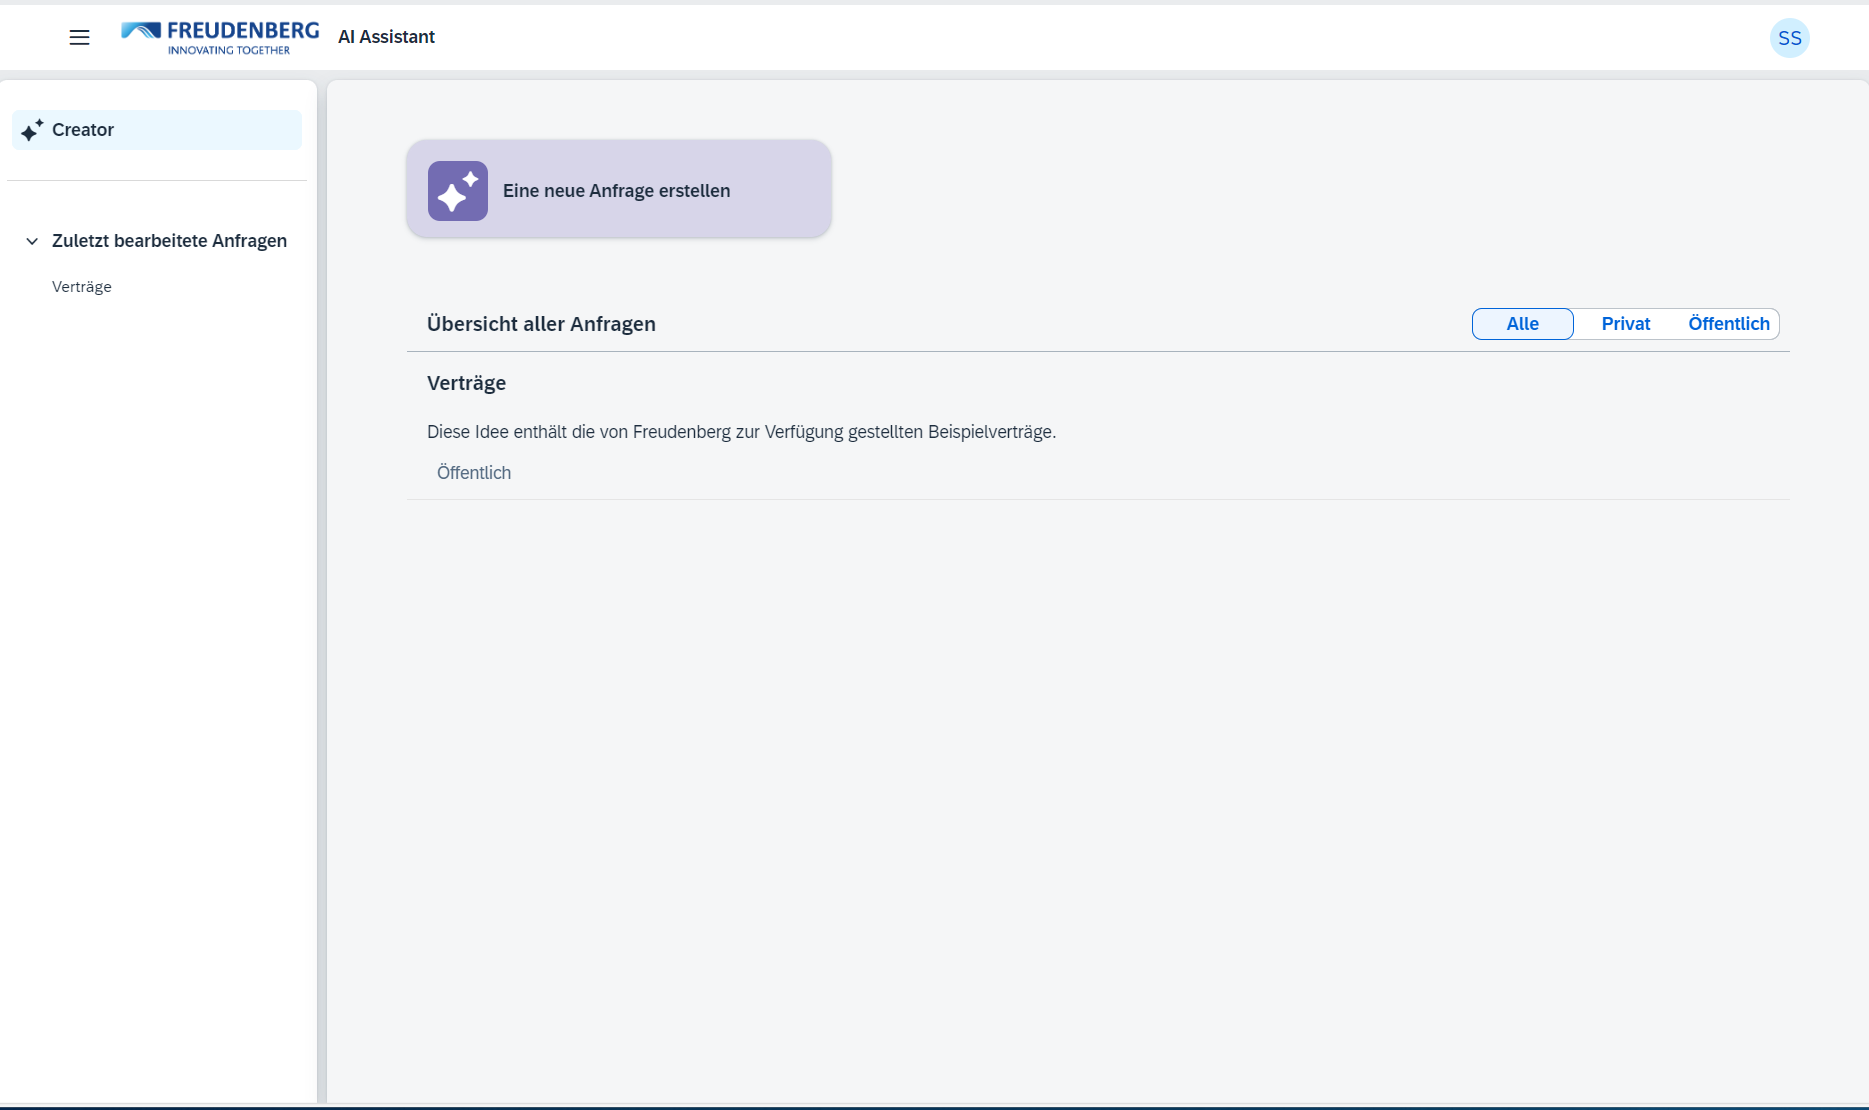
\includegraphics[width=1\textwidth]{img/Chatbot_start.png}
    \caption{AI Assistant Startseite}
    \label{fig:chatbot_start}
\end{figure}

Klickt der Benutzer auf „Eine neue Anfrage erstellen“, gelangt er zur Upload-Seite, auf der beliebig viele PDF-Dokumente hochgeladen werden können, 
die in den Kontext der Anfrage eingebunden werden (siehe Abbildung \ref{fig:neue_anfrage}). 

Im Hintergrund werden die hochgeladenen PDF-Dokumente zunächst in einem File Storage gespeichert. Ein PDF Reader liest dann die hochgeladenen Dateien aus und erstellt relevante Metadaten, 
wie die Kontext-ID und Dokument-ID. Diese Metadaten dienen dazu, die Dokumente zu verwalten und sie nach der Verarbeitung in Chunks korrekt zuzuweisen.

Nach der Extraktion der Metadaten werden die PDF-Dokumente in Chunks unterteilt. Diese Chunks werden dann durch das Embedding-Modell \textit{multilingual-e5-large} in Vektoren umgewandelt. 
Diese Vektoren werden anschließend in einer Vektor-Datenbank gespeichert, wobei sie mit der Kontext-ID verknüpft sind, um die Zuordnung der Chunks zu einem bestimmten Kontext zu gewährleisten. 
Die Vektor-Datenbank ermöglicht so die semantische Suche.

Sobald der Benutzer eine Anfrage an den Chatbot stellt, wird der Prompt zusammen mit der zugehörigen Kontext-ID abgesendet. 
LlamaIndex übernimmt dann die Verarbeitung des Prompts, nachdem dieser ebenfalls mithilfe des Embedding-Modells in einen Vektor umgewandelt wurde. 
Hierbei führt LlamaIndex eine Similarity-Suche in der Vektor-Datenbank durch, wobei nur die Einträge mit derselben Kontext-ID berücksichtigt werden. 
Auf diese Weise werden die am besten passenden Chunks der hochgeladenen Dokumente identifiziert.

Diese relevanten Chunks werden aus der Vektor-Datenbank geladen und zusammen mit dem Prompt über SAP AI Core an das \ac{LLM} \textit{LLaMA3-70b} gesendet. 
Die Verbindung zu SAP AI Core erfolgt über das Python SAP AI Core \ac{SDK}, das es ermöglicht, die Prompts und die Chunks effizient an das \ac{LLM} zu übermitteln. 
Das \ac{LLM} verarbeitet diese Informationen und generiert auf Basis des Prompts und der relevanten Chunks eine Antwort, die dann an den Benutzer zurückgegeben wird. 
Durch diesen Ablauf wird sichergestellt, dass der Chatbot nicht nur schnelle, sondern auch kontextuell passende und präzise Antworten liefern kann.


\begin{figure}[H]
    \centering
    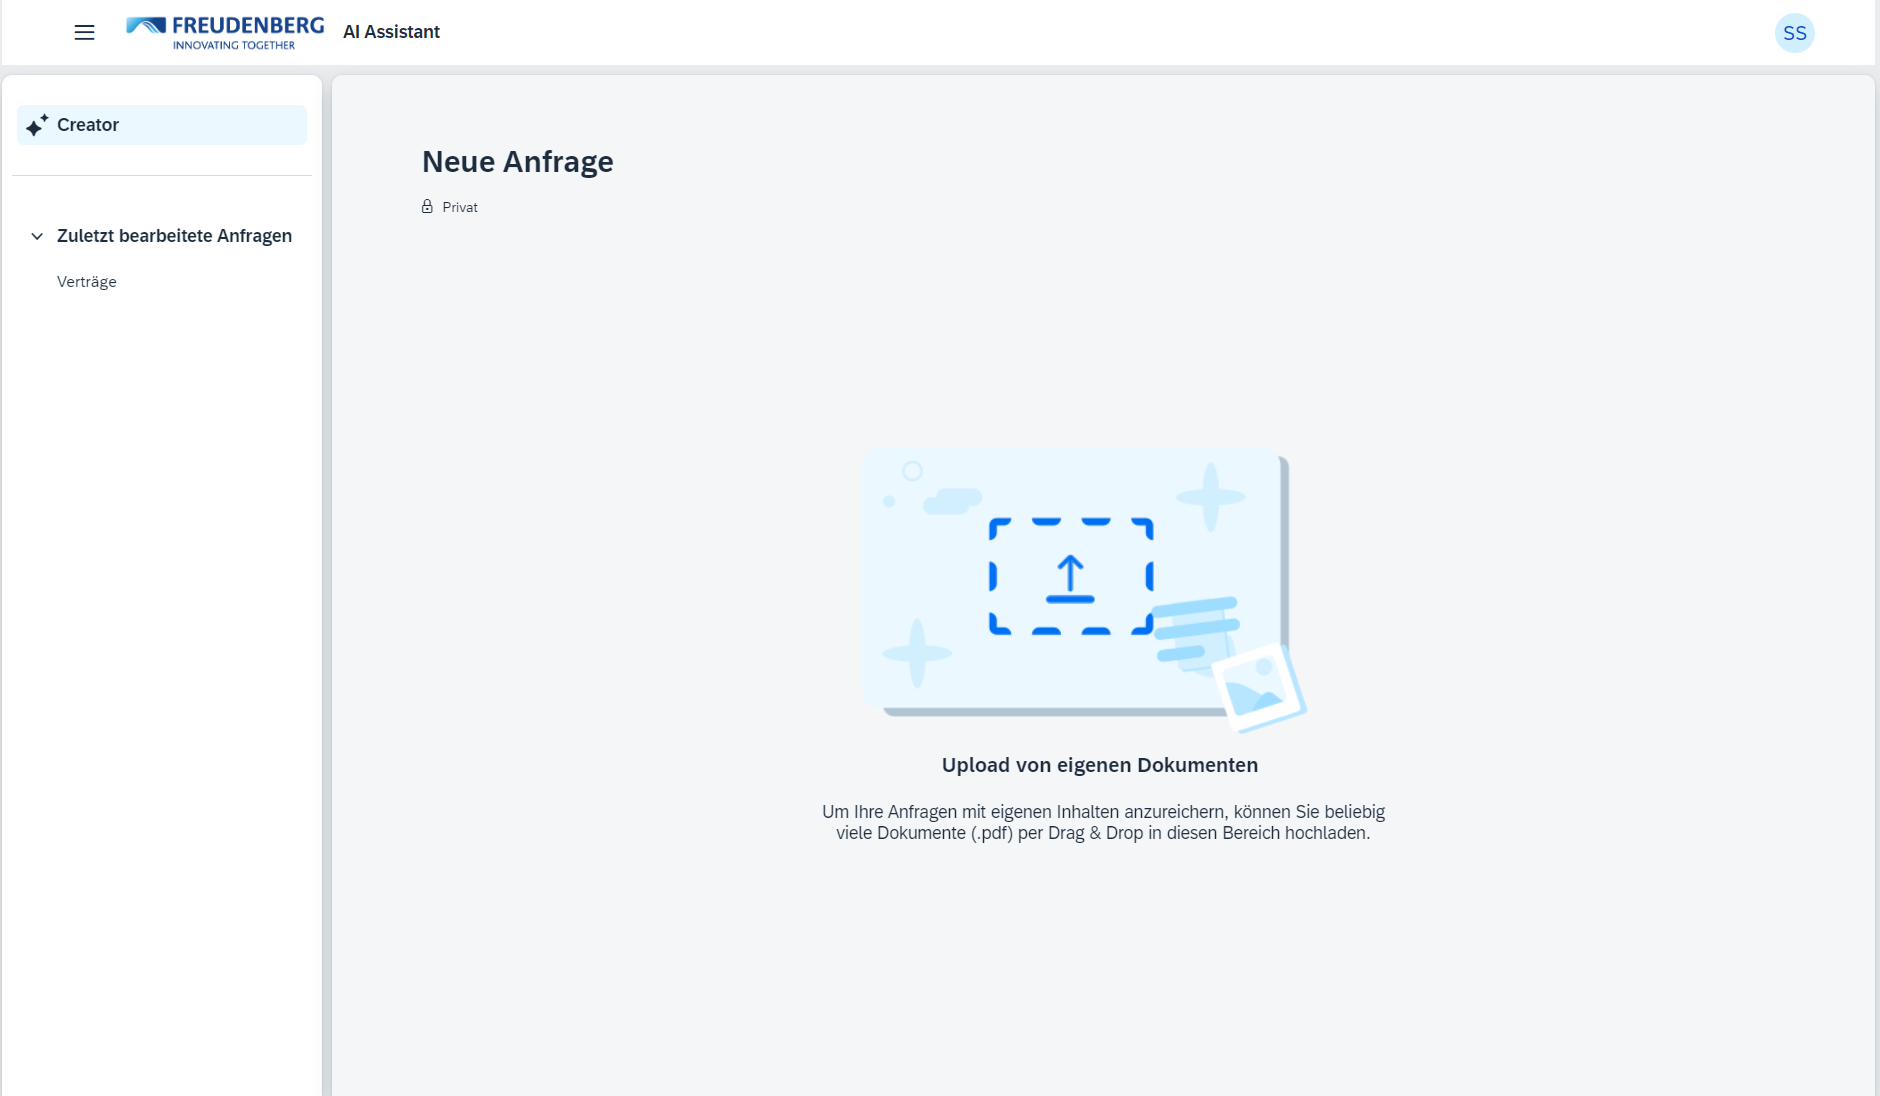
\includegraphics[width=1\textwidth]{img/Chatbot_neue_Anfrage.png}
    \caption{Eine neue Anfrage erstellen}
    \label{fig:neue_anfrage}
\end{figure}

\subsection{Zugriff auf bestehende Anfrage}

Außer eine neue Anfrage anzulegen kann der Benutzer auch auf bestehende Anfragen zugreifen, z. B. auf die öffentlich erstellte Anfrage „Verträge“ (siehe Abbildung \ref{fig:chatbot_vertraege_leer}). 
Der Kontext dieser Anfrage umfasst 12 Verträge der Freudenberg Gruppe, darunter \acp{NDA} und andere geschäftliche Verträge. Vertrauliche Daten in den Dokumenten wurden für die Arbeit geschwärzt. 

Diese Anfrage wurde vorab als Beispiel in den AI Assistant integriert, um den Benutzern die Möglichkeit zu geben, sich mit den Funktionen des Tools vertraut zu machen. 

\begin{figure}[H]
    \centering
    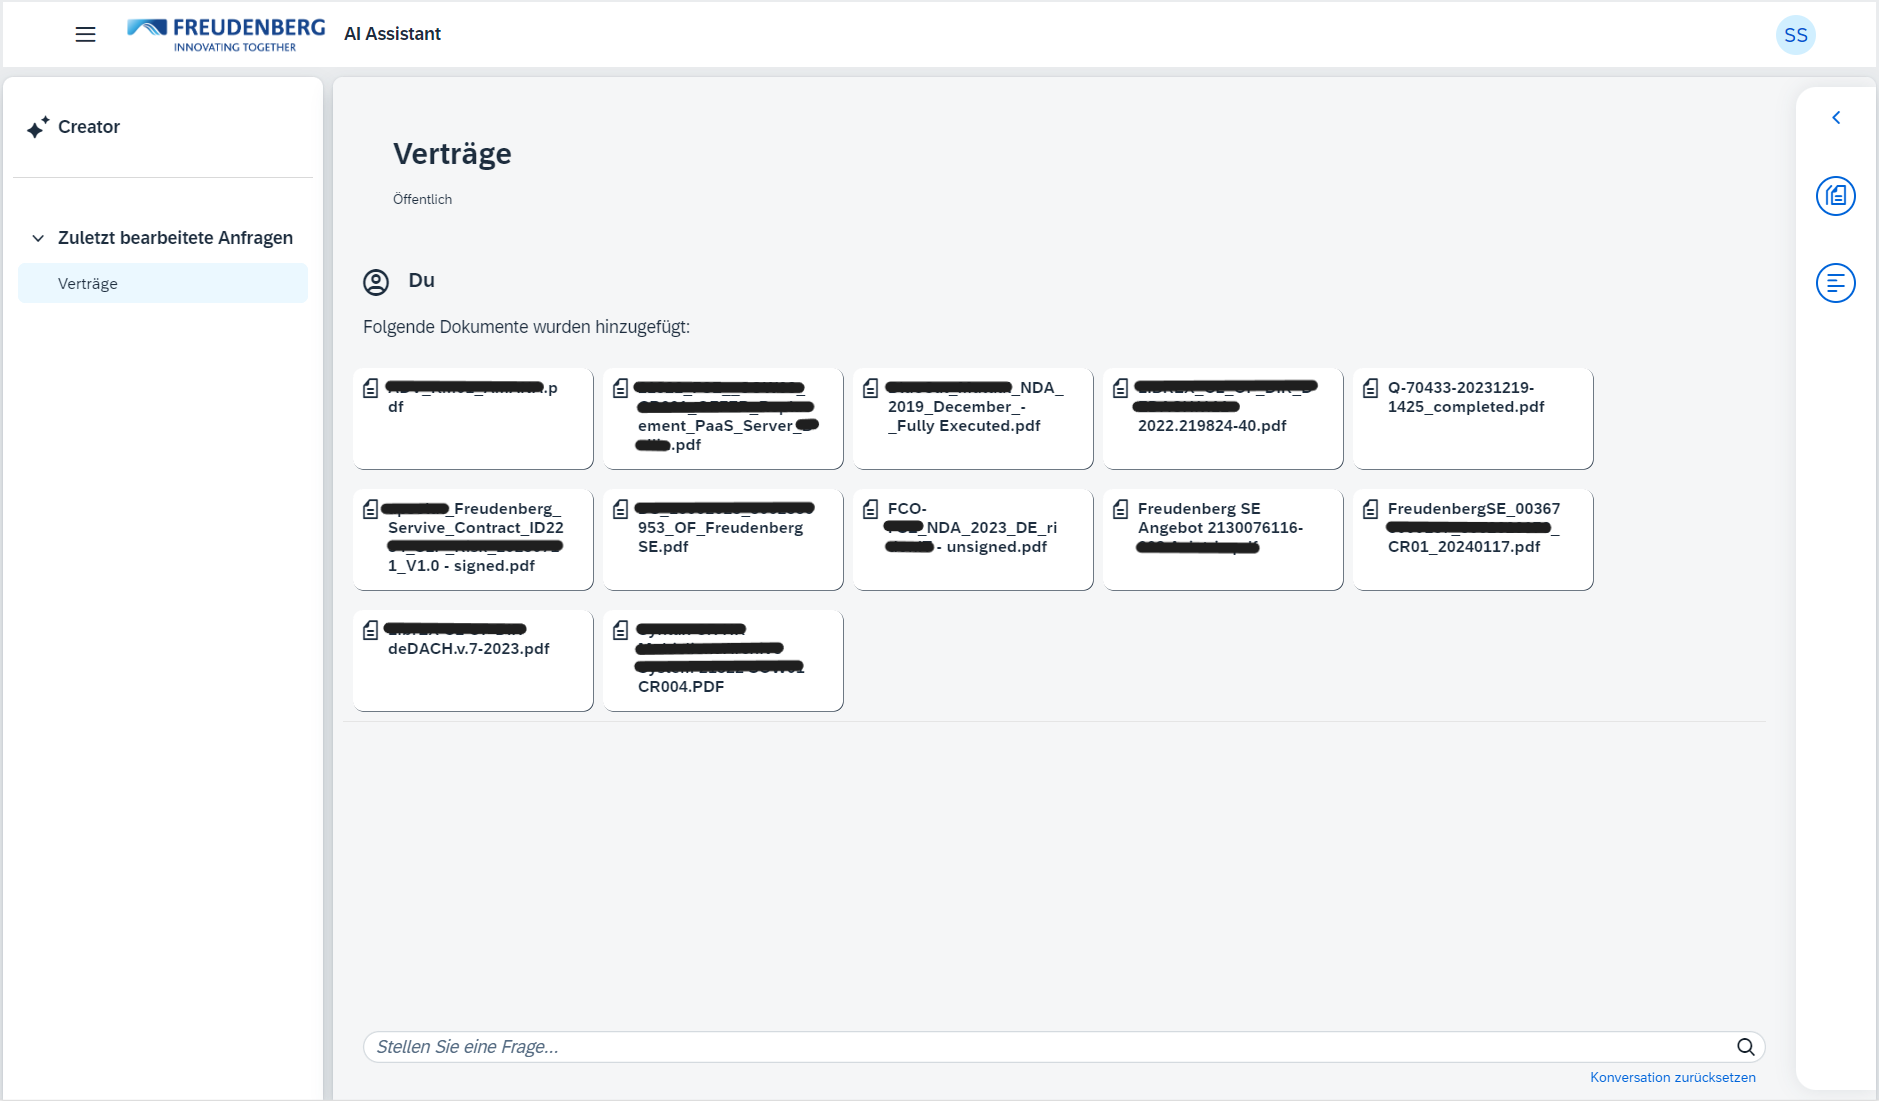
\includegraphics[width=1\textwidth]{img/Chatbot_vertraege_leer.png}
    \caption{Anfrage „Verträge“ mit vorbereitetem Kontext}
    \label{fig:chatbot_vertraege_leer}
\end{figure}

Benutzer können spezifische Fragen zu den Verträgen stellen, woraufhin der Chatbot den Prompt mithilfe des Embedding-Modells \textit{multilingual-e5-large} in einen Vektor umwandelt und zusammen mit der Kontext-ID an LlamaIndex sendet. 
LlamaIndex führt eine Similarity-Suche in der Vektor-Datenbank durch, wobei nur die Einträge mit derselben Kontext-ID berücksichtigt werden. 
Die am besten passenden Chunks werden anschließend gemeinsam mit dem Prompt an das \ac{LLM} gesendet. 

Nach der Verarbeitung durch das \ac{LLM} erhält der Chatbot sowohl die Antwort auf die Anfrage als auch die Top-K-Menge, hier 20, der relevantesten Chunks. 
Diese Chunks werden dem Benutzer zusammen mit der Antwort angezeigt (siehe Abbildung \ref{fig:chatbot_vertraege_anfrage}), um ihm zu ermöglichen, die Quellen der Informationen nachzuvollziehen. 
Diese Funktion dient als zusätzliche Sicherheit, damit die Benutzer überprüfen können, aus welchen Dokumenten die Informationen stammen und ob sie korrekt sind.

In Abbildung \ref{fig:chatbot_vertraege_anfrage} wird eine Frage zu den Inhalten eines \ac{NDA} mit einem externen Partner gestellt, und der AI Assistant antwortet mit den Informationen, die dem \ac{NDA} zu entnehmen sind. 
Rechts in der Seitenleiste werden die relevanten Textstellen markiert, die aus den eingebetteten Verträgen extrahiert wurden. 
Dies zeigt die Fähigkeit des Chatbots, semantische Suchen durchzuführen und präzise Informationen aus dem relevanten Vertrag im gespeicherten Kontext zu extrahieren.

\begin{figure}[H]
    \centering
    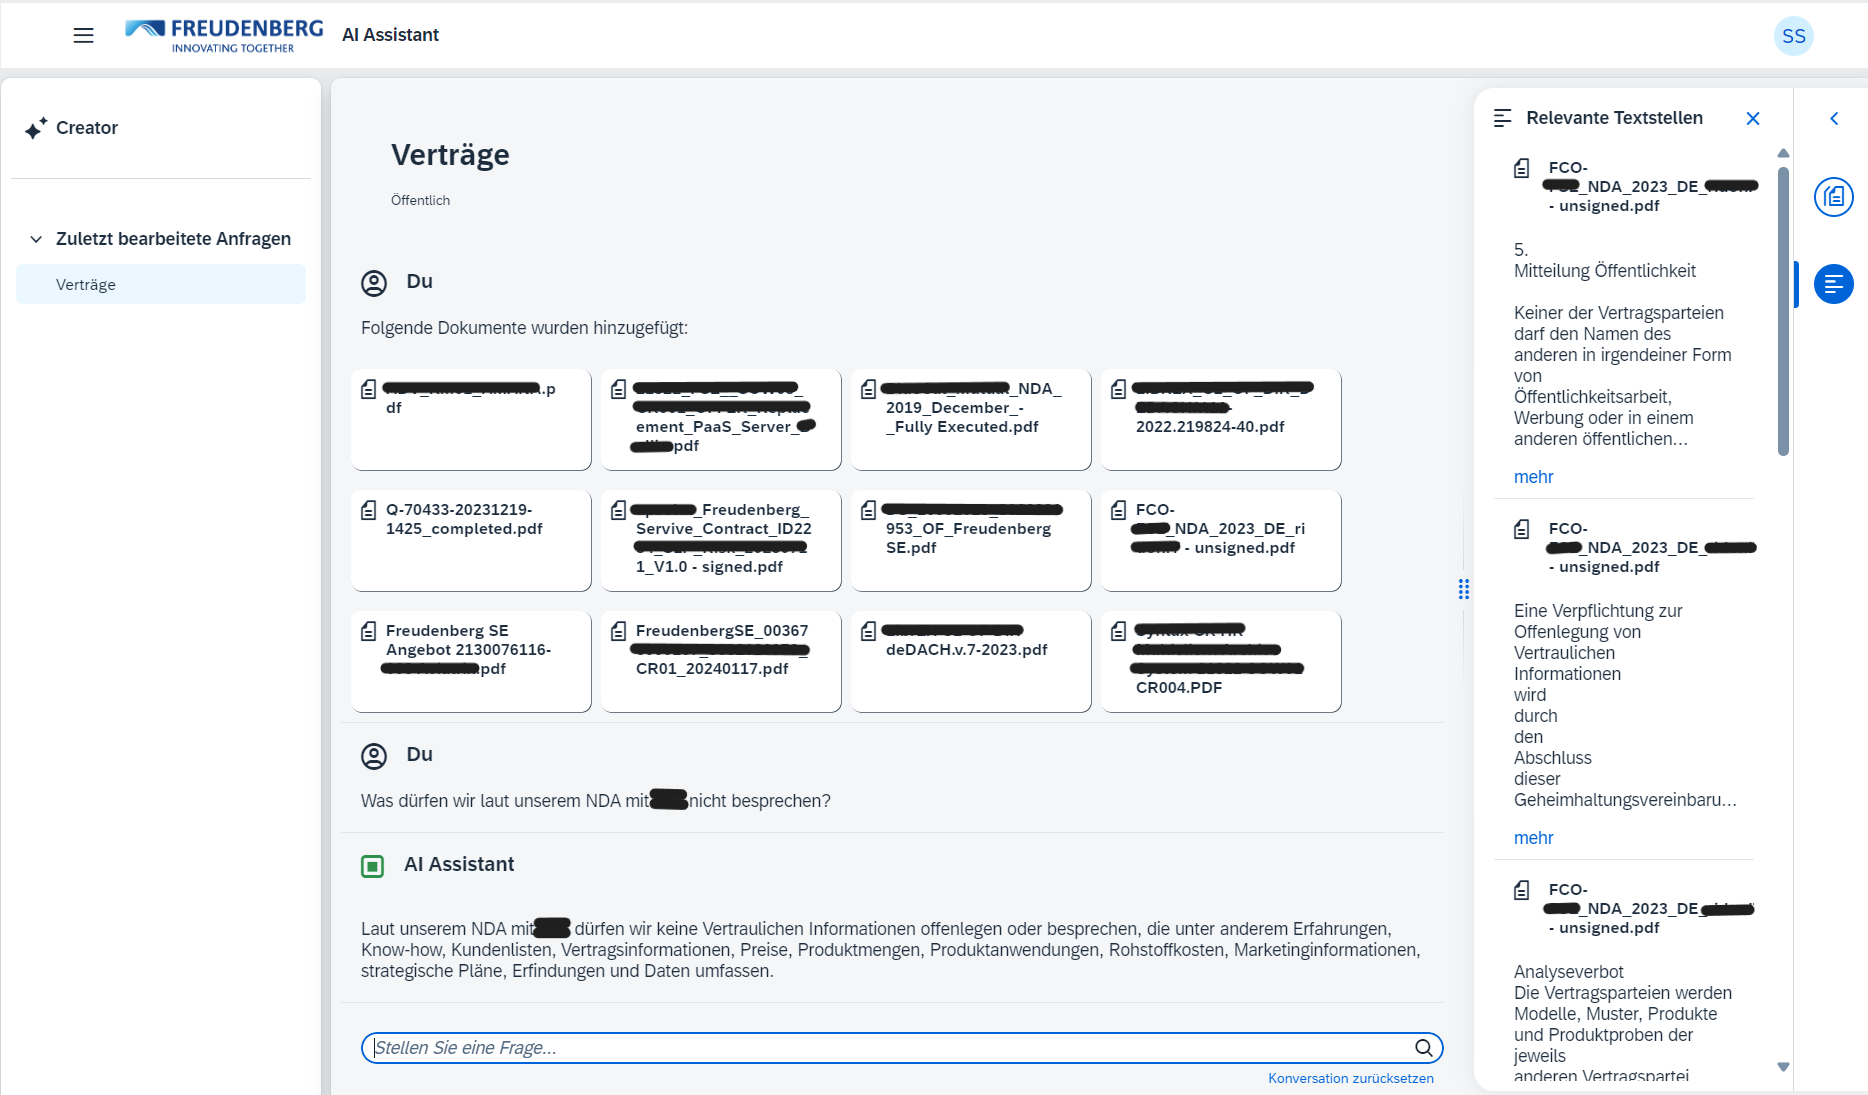
\includegraphics[width=1\textwidth]{img/Chatbot_vertraege_anfrage.png}
    \caption{Beispiel einer Anfrage zu Verträgen}
    \label{fig:chatbot_vertraege_anfrage}
\end{figure}

\subsection{Verlauf und Speicherfunktionalität}

Der AI Assistant kann zudem den gesamten Gesprächsverlauf für zukünftige Anfragen nutzen. In Abbildung \ref{fig:memory_proof} wird ein Beispiel gezeigt, 
in dem der Benutzer den Chatbot nach einem Angebot eines Vertragspartners fragt. Nachdem der Chatbot die Frage beantwortet hat, stellt der Benutzer eine neue Frage: „Was war nochmal meine Frage?“ 
Der Chatbot ist in der Lage, auf den Gesprächsverlauf zuzugreifen und korrekt zu antworten, indem er die ursprüngliche Frage wiedergibt. 
Dies wird ermöglicht, indem der gesamte Chatverlauf zur Laufzeit an das \ac{LLM} geschickt wird.

\begin{figure}[H]
    \centering
    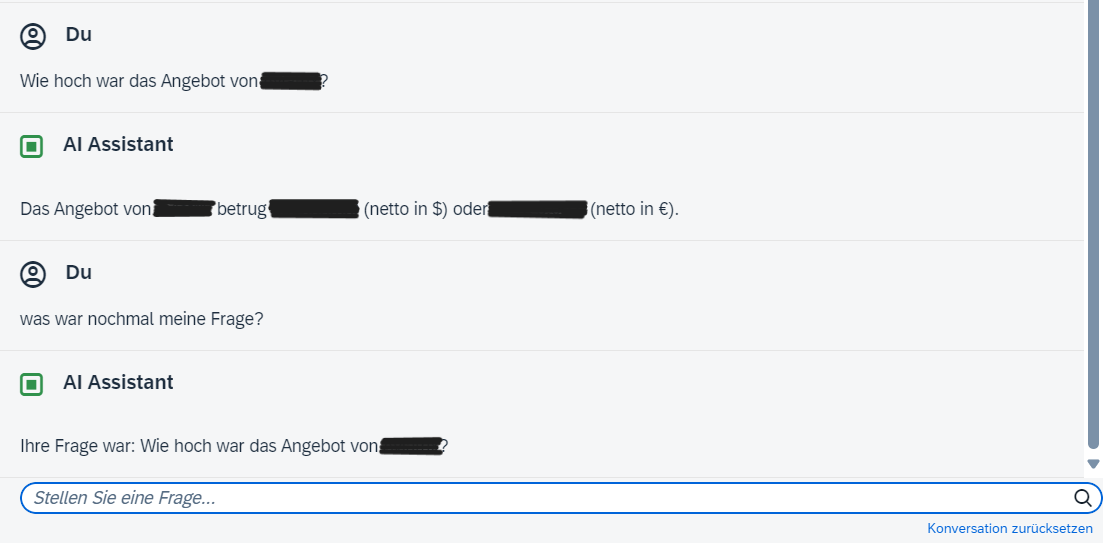
\includegraphics[width=1\textwidth]{img/Chatbot_memory_proof.png}
    \caption{Beweis für die Nutzung des Chatverlaufs}
    \label{fig:memory_proof}
\end{figure}

Zusätzlich wird in Abbildung \ref{fig:memory_use} ein weiteres Beispiel für die Gedächtnisfunktionalität gezeigt. Der Benutzer fragt den AI Assistant zuerst dieslbe Frage nach dem Angebot eines Vertragspartners 
und erhält dieselbe detaillierte Antwort. Anschließend stellt er eine Folgefrage: „Aus welchem Jahr?“ ohne das ursprüngliche Angebot erneut zu erwähnen. 
Der AI Assistant antwortet korrekt mit dem Jahr und dem exakten Datum des Angebots. Diese Funktionalität verbessert die Benutzerfreundlichkeit erheblich, 
da der Benutzer in der Lage ist, mehrere zusammenhängende Fragen zu stellen, ohne den gesamten Kontext wiederholen zu müssen. 
Dies ermöglicht präzisere und effizientere Konversationen, insbesondere bei komplexen Sachverhalten.

\begin{figure}[H]
    \centering
    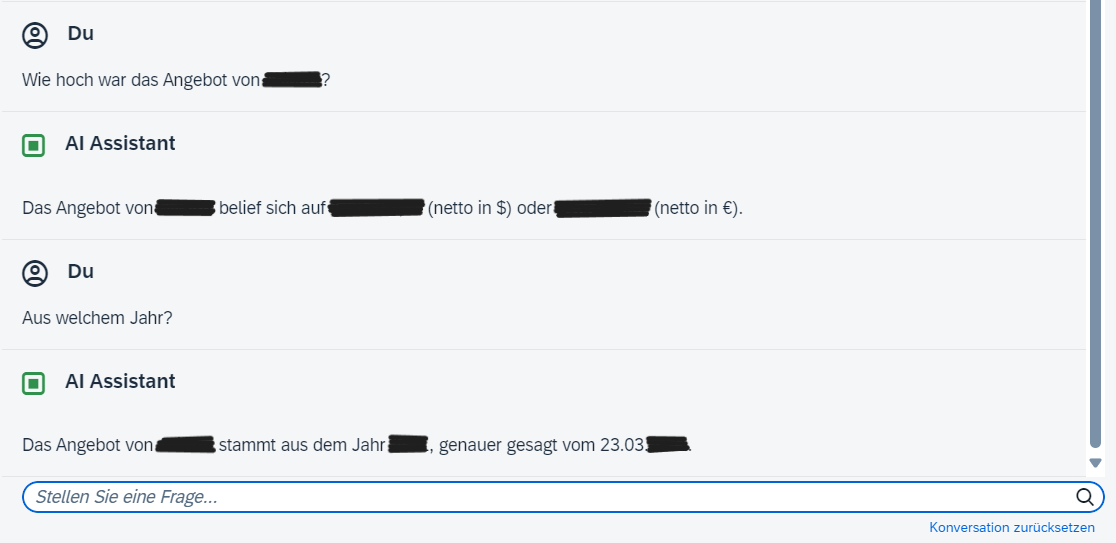
\includegraphics[width=1\textwidth]{img/Chatbot_memory_use.png}
    \caption{Nutzung des Chatverlaufs für präzisere Folgefragen}
    \label{fig:memory_use}
\end{figure}
\cleardoublepage
% Fazit und Ausblick
\chapter{Fazit und Ausblick}
\label{fazit}

\nocite{*}

In diesem Kapitel werden die wesentlichen Ergebnisse der Untersuchung zusammengefasst und kritisch reflektiert. Darüber hinaus wird ein Ausblick auf zukünftige Entwicklungen des AI Assistant bei Freudenberg \& Co. KG (\ac{FCO}) gegeben. 

\section{Zusammenfassung der Ergebnisse}

Im Rahmen dieser Arbeit wurde die Entwicklung eines \ac{KI}-basierten Chatbots, dem AI Assistant für Freudenberg \& Co. KG (\ac{FCO}), erfolgreich umgesetzt. 
Die zentrale Grundlage dafür bildete die detaillierte Evaluation von Large Language Models (\acp{LLM}) und Embedding-Modellen, die im Kontext von SAP AI Core getestet wurden, um eine effiziente und präzise Lösung zu entwickeln.

Die Evaluation \ref{eval_llm} der \acp{LLM} ergab, dass \textit{GPT-3.5-Turbo} in der Gesamtbewertung die besten Leistungen zeigte, insbesondere hinsichtlich Antwortqualität und Antwortzeit. 
\textit{LLaMA3-70b} erwies sich als das leistungsstärkste Open-Source-Modell und wurde für den Einsatz im AI Assistant gewählt, da es eine vergleichsweise hohe Qualität bot und den zusätzlichen Anforderungen an Datenschutz und interne Kontrolle gerecht wurde.

Laut der Evaluation \ref{eval_embedding} der Embedding-Modellen schnitt \textit{multilingual-e5-large} am besten unter den Open-Source-Optionen ab, insbesondere in Bezug auf die Identifikation relevanter Textstellen in großen Dokumenten. 
Auch wenn \textit{text-embedding-3-large} in der Untersuchung technisch die besten Ergebnisse lieferte, wurde \textit{multilingual-e5-large} aufgrund der Open-Source-Anforderungen bevorzugt.

Ein wesentlicher Befund der Untersuchung war, dass sich die getesteten \acp{LLM} hinsichtlich ihrer Leistung deutlich voneinander unterschieden. 
Besonders auffällig war dabei die Sensibilität der Modelle gegenüber den Parametern \textit{chunk size} und \textit{top k}. 
Je nach gewählter Konfiguration konnten sich die Bewertungsergebnisse der Modelle in der Skala von 0 bis 10 um bis zu 4 Punkte unterscheiden. 
Diese Erkenntnis verdeutlicht die Notwendigkeit, spezifische Parameter sorgfältig anzupassen, um die optimale Leistung eines Modells im AI Assistant zu gewährleisten.

Der AI Assistant konnte erfolgreich implementiert werden und zeigt eine hohe Leistungsfähigkeit bei der Verarbeitung von Anfragen, die auf eingebetteten Dokumenten basieren. 
Durch die Kombination von \textit{LLaMA3-70b} und \textit{multilingual-e5-large} in Verbindung mit LlamaIndex gelingt es dem Chatbot, präzise Antworten auf der Grundlage relevanter Textstellen zu generieren. 
Dabei spielen insbesondere die Einbettung großer Dokumentensammlungen und die Verwaltung des Kontexts über den gesamten Chatverlauf hinweg eine entscheidende Rolle. 
Die Implementierung einer Gedächtnisfunktionalität und die Anzeige der Top-K-Chunks als zusätzliche Funktion tragen zur Benutzerfreundlichkeit und Nachvollziehbarkeit der Ergebnisse bei. 
Benutzer können so jederzeit die Herkunft und Relevanz der präsentierten Informationen überprüfen, was die Effizienz des Assistants weiter steigert.

Insgesamt zeigen die Ergebnisse, dass der AI Assistant durch die ausgewählten Open-Source-Modelle und die technische Umsetzung eine leistungsstarke und flexible Lösung bietet, die den Anforderungen von \ac{FCO} gerecht wird.

\section{Zukunftsausblick}

Zukünftig können immer neuere und leistungsfähigere \acp{LLM} über SAP AI Core in den AI Assistant integriert werden, um die Antwortqualität des Chatbots kontinuierlich zu verbessern. 
Es ist daher essenziell, dass die Corporate IT (\ac{CIT}) bei jedem neuen Modell, das der \ac{BTP} hinzugefügt wird, eine erneute Evaluation durchführt, um sicherzustellen, dass stets das bestmögliche Modell zum Einsatz kommt. 
Darüber hinaus liegt es in der Verantwortung der Administratoren des AI Assistant, hochwertige öffentliche Kontexte bereitzustellen, 
die allgemein relevante Informationen bieten und den Mitarbeitern eine umfassende Unterstützung ermöglichen.

Um die Benutzerfreundlichkeit weiter zu erhöhen, wäre es vorteilhaft, unterschiedliche Nutzergruppen einzurichten, sodass gezielt zugeschnittene Kontexte zur Verfügung gestellt werden können. 
Auf diese Weise könnten beispielsweise die Rechtsabteilung und die Cyber-Security-Abteilung jeweils nur auf für sie relevante Kontexte zugreifen, wodurch die Effizienz gesteigert und die Übersichtlichkeit verbessert wird.

Langfristig könnte der AI Assistant auf weitere Geschäftsbereiche ausgeweitet werden, um gruppenweit die Vorteile der \ac{KI}-Implementierung zu nutzen. 
Ein zusätzlicher Ansatz zur Optimierung des Chatbots liegt in der gezielten Steigerung der Dokumentenqualität. 
So könnten beispielsweise Strategien entwickelt werden, um die Qualität von Meeting-Protokollen und anderen internen Dokumenten durch Schulungen und Standards zu verbessern, 
sodass diese für den Chatbot besser nutzbar sind und zu präziseren Antworten beitragen.

\section{Lessons Learned}

Im Verlauf der Evaluation und Implementierung des AI Assistant traten verschiedene Herausforderungen auf, insbesondere bei der Erfassung und Speicherung der Messdaten. 
Als erstes gab es Schwierigkeit bei der Sicherung der Umfrageergebnisse, die für die Gewichtung der Bewertungsfaktoren in der Score Function verwendet wurden. 
Während die Antworten erfolgreich in einer Excel-Datei erfasst wurden, kam es im Backup-Prozess zu einem irreversiblen Datenverlust der Rohdaten. 
Dieses Ereignis verdeutlichte die Notwendigkeit robuster und redundanter Sicherungsstrategien, insbesondere bei Daten, die für zukünftige Anpassungen und Bewertungen von zentraler Bedeutung sind.

Ein weiteres Problem ergab sich bei der Evaluation der Embedding-Modelle. Während die Ergebnisse für die Large Language Models (LLMs) umfassend dokumentiert und gesichert werden konnten, 
wurden die Ergebnisse der Embedding-Modelle lediglich im Vergleich zueinander gespeichert, ohne absolute Werte zu erfassen. 
Diese Entscheidung führte später zu Schwierigkeiten bei der transparenten Darstellung der genauen Ergebnisse. 
Da auf den ursprünglichen Rechner, auf dem die Evaluation durchgeführt wurde, kein Zugriff mehr besteht, konnten die exakten Werte nicht nachträglich gesichert werden.

Zusätzlich wurde festgestellt, dass auch für die LLMs nur die Endergebnisse in Form von Grafiken und aggregierten Auswertungen gesichert wurden, ohne die vollständigen Rohdaten zu speichern. 
In Zukunft ist es daher ratsam, sämtliche Rohdaten systematisch zu archivieren, um bei Bedarf auf alle Messwerte und Details zugreifen zu können.

Zusammenfassend zeigen diese Erfahrungen, dass eine klare und umfassende Datenspeicherstrategie von Anfang an notwendig ist, um Datenverluste zu vermeiden und eine nachhaltige Verfügbarkeit der Evaluationsdaten sicherzustellen. 
Dies ist besonders wichtig, da zukünftige Iterationen des Projekts sowie mögliche Reevaluierungen der Modelle auf eine verlässliche Datengrundlage angewiesen sind.
%%%%%%%%%%%%%%%%%%%%%%%%%%%%%%%%%%%

%%%%%%%%%%%%%%%%%%%%%%%%%%%%%%%%%%%
% ANHÄNGE
%
% @stud: einzelne Anhänge bearbeiten und eigene Anhänge hier einfügen 
%        die nachfolgenden Zeilen deaktivieren, wenn keine Anhänge verwendet werden
%
\initializeAppendix
% \input{appendix1}

% \input{appendix2}
%%%%%%%%%%%%%%%%%%%%%%%%%%%%%%%%%%%

\singlespacing

\setlength{\bibitemsep}{1.5em}

%\ihead{}
%\printbibliography[title=\Literaturverzeichnis] 
\printbibliography 
\cleardoublepage

%\initializeBibliography
%%%%%%%%%%%%%%%%%%%%%%%%%%%%%%%%%%%

%%%%%%%%%%%%%%%%%%%%%%%%%%%%%%%%%%%
% INDEX
% @stud: ggf. Index auskommentieren, wenn nicht benötigt
%
% \addcontentsline{toc}{chapter}{Index}
% \printindex

\end{document}